\documentclass{report}
\usepackage[T1]{fontenc} % Fontes T1
\usepackage[utf8]{inputenc} % Input UTF8
\usepackage[backend=biber, style=ieee]{biblatex} % para usar bibliografia
\usepackage{csquotes}
\usepackage[portuguese]{babel} %Usar língua portuguesa
\usepackage{blindtext} % Gerar texto automaticamente
\usepackage[printonlyused]{acronym}
\usepackage{hyperref} % para autoref
\usepackage{graphicx}
\usepackage{float}

\bibliography{bibliografia}


\begin{document}
%%
% Definições
%
\def\titulo{Adivinha o Número Secreto}
\def\data{30/05/2020}
\def\autores{Mauro Marques Canhão Filho, Patricia Rafaela da Rocha Cardoso }
\def\autorescontactos{(103411) mauro.filho@ua.pt, (103243) patriciarcardoso@ua.pt}
\def\versao{1.0}
\def\departamento{Departamento de Eletrônica, Telecomunicações e Informática (DETI)}
\def\empresa{Universidade de Aveiro}
\def\logotipo{ua.pdf}
%
%%%%%% CAPA %%%%%%
%
\renewcommand{\contentsname}{Índice}
\begin{titlepage}

\begin{center}
%
\vspace*{50mm}
%
{\Huge \titulo}\\ 
%
\vspace{10mm}
%
{\Large \empresa}\\
%
\vspace{10mm}
%
{\LARGE \autores}\\ 
%
\vspace{30mm}
%
\begin{figure}[h]
\center
\includegraphics{\logotipo}
\end{figure}
%
\vspace{30mm}
\end{center}
%
\begin{flushright}
\versao
\end{flushright}
\end{titlepage}

%%  Página de Título %%
\title{%
{\Huge\textbf{\titulo}}\\
{\Large \departamento\\ \empresa}
}
%
\author{%
    \autores \\
    \autorescontactos
}
%
\date{\data}
%
\maketitle

\pagenumbering{roman}

%%%%%% RESUMO %%%%%%
\begin{abstract}
Este relatório tem como objetivo descrever a implementação e a intereção entre um servidor e um ou mais clientes. Para isso, será detalhadamente apresentado o funcionamento/criação de um jogo. O jogo consiste em o cliente adivinhar um número inteiro aleatório entre 0 e 100, o número secreto, gerado aleatoriamente pelo servidor.Serão detalhadamente descritos o programa cliente e o programa servidor e a criptogafia a eles associados bem como o funcionamento criação e desenvolvimento de testes funcionais e unitários. Com base em imagens de todas as funções em ambos os programas e imagens da intereção no terminal entre um ou mais clientes e o servidor é possível perceber o funcionamento correto da aplicação.
\end{abstract}

\tableofcontents
% \listoftables     % descomentar se necessário
 \listoffigures    % descomentar se necessário


%%%%%%%%%%%%%%%%%%%%%%%%%%%%%%%
\clearpage
\pagenumbering{arabic}

%%%%%%%%%%%%%%%%%%%%%%%%%%%%%%%%
\chapter{Introdução}
\label{chap.introducao}
O objetivo deste trabalho é explicar,enumerar e descrever o desenvolvimento e funcionamento de um servidor que suporte a geração de um número inteiro aleatório (entre 0 e 100), o número secreto, bem como o número máximo de tentativas (entre 10 e 30) concedidas para o adivinhar. E um cliente que permita adivinhar esse número secreto. Ou seja um jogo de adivinha o número secreto.
O servidor nunca deverá aceitar dois clientes com a mesma identificação a jogar simultaneamente e deverá criar e atualizar um ficheiro designado por report.csv onde vai escrevendo os resultados dos diversos clientes quando estes terminam o jogo. O cliente pode desistir em qualquer altura e o jogo acaba quando ele adivinha o número secreto ou quando esgota o número máximo de tentativas que dispunha para jogar. Caso o cliente exceda o número de jogadas de que dispunha o jogo será considerado sem sucesso mesmo que ele tenha adivinhado o número. Quando o jogo acaba corretamente o cliente deve escrever no monitor uma mensagem a indicar se adivinhou ou não o número secreto e quantas jogadas efectuou. Por sua vez o servidor acrescenta ao ficheiro a informação relativa ao jogo: cliente; número secreto; número máximo de jogadas; número de jogadas efectuadas; e o resultado obtido pelo cliente (desistência ou sucessso ou insucessso).
Também será abordado e aprofundado o conceito de criptogafia e a realização e funcionamento de testes funcionais e unitários bem como a explicação detalhada do desenvolvimento da aplicação.


\chapter{Metodologia}
\label{chap.metodologia}
Neste capítulo será detalhadamente descrito o algoritmo e o funcionamento do progama servidor e do programa cliente bem como a implementação dos testes funcionais e unitários.
\section{Servidor}
O programa servidor consiste em gerar aleatoriamente um número entre 0 e 100 e um número máximo de tentativas entre 10 e 30 para o adivinhar. 
	O programa servidor é constítuido por um dicionário e as seguintes funções: \textbf{find\_client\_id},\textbf{encrypt\_intvalue}, \textbf{decrypt\_intvalue}, \textbf{new\_msg}, \textbf{numberToCompare}, \textbf{new\_client}, \textbf{clean\_client}, \textbf{quit\_client}, \textbf{create\_file}, \textbf{update\_file}, \textbf{guess\_client}, \textbf{stop\_client} e \textbf{main}.
\subsection{Armazenamento dos resultados num ficheiro csv}
\begin{figure}[H]
        \centering
        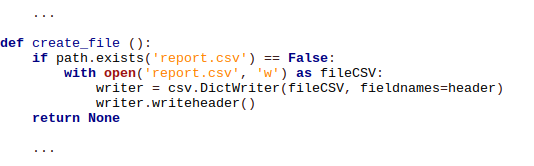
\includegraphics[scale=0.65]{create_file}       
        \caption{Função que cria um ficheiro report.csv quando o servidor é inicializado.}
\end{figure}
No momento em que o servidor é inicializado é chamada a função "create\_file" para que seja criado um novo ficheiro report.csv caso ainda não exista no diretório em que o server.py se encontra. Assim, o servidor não reinicia o ficheiro sempre que for inicializado. Depois, escreve o cabeçalho no ficheiro com base no array "header".O array "header" é utilizado para atualizar o cabeçalho do ficheiro report.csv que será gerado pelo servidor.
\begin{figure}[H]
        \centering
        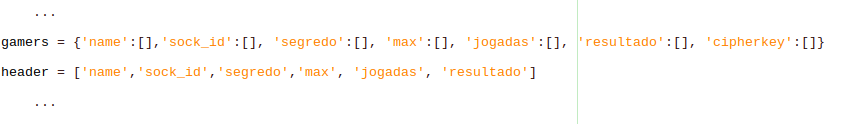
\includegraphics[scale=0.65]{dicionarioearray_server}   
        \caption{Dicionário constituído pelos dados dos jogadores e array responsável pela inicialização do header no ficheiro report.csv.}
\end{figure}
Por outro lado, o dicionário "gamers" armazena os dados dos jogadores que estão atualmente com um jogo iniciado. A informação armazenada é baseada na ordem pela qual os clientes se conectam ao servidor. Essa informação é filtrada e distribuída por arrays que contém diferentes campos de identificação. Por exemplo, se dois jogadores, Mauro e Patrícia estiverem a jogar simultaneamente e se o Mauro se conectou primeiro ao servidor, o seu ID pode ser consultado através de: gamers['sock\_id'][0], enquanto o ID da Patrícia pode ser acedido da seguinte forma: gamers['sock\_id'][1].

\begin{figure}[H]
        \centering
        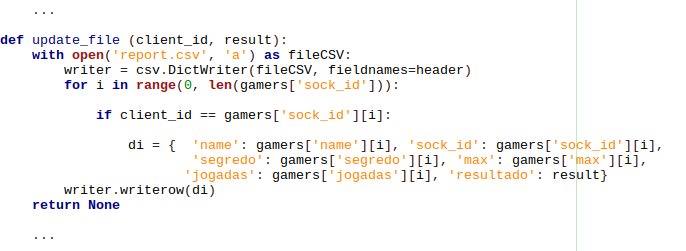
\includegraphics[scale=0.65]{update_file}       
        \caption{Função que atualiza o ficheiro report.csv quando um jogo é terminado.}
\end{figure}

Quando um jogo termina com sucesso, sem sucesso ou em caso de desistência é chamada a função "update\_file" que atualiza o ficheiro report.csv com os dados do jogador.Para isso, abre o ficheiro no modo "a" (append) para adicionar dados sem escrever sobre aqueles que já lá estavam.Assim, procura pelo index "i" tal que o sock\_id é igual ao client\_id passado como parâmetro da função. Por fim, escreve todos os itens na posição "i" dos arrays do dicionário "gamers" no ficheiro report.csv. 

\subsection{Funcionamento geral do jogo}
\begin{figure}[H]
        \centering
        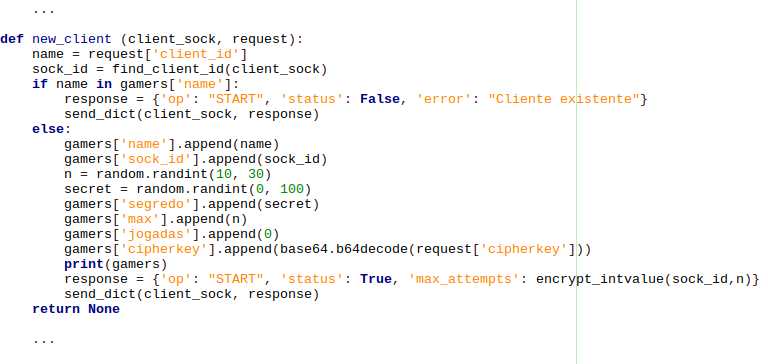
\includegraphics[scale=0.65]{new_client}        
        \caption{Função que cria um novo cliente no jogo.}
\end{figure}
O jogo é iniciado quando o servidor recebe uma mensagem do cliente com o comando "START" tornando-se num jogador ativo e provocando as seguintes ações no servidor:
\begin{enumerate}
\item Armazenamento na variável "name" do "client\_id" passado para o servidor aquando da inserção pelo utilizador na linha de comandos ao executar o cliente;
\item Identificação do ID(porto ao qual está conectado) do cliente a partir do socket recorrendo à função "find\_client\_id";

\begin{figure}[H]
        \centering
        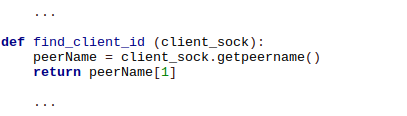
\includegraphics[scale=0.65]{find_client_id}    
        \caption{Função que retorna o porto ao qual o cliente está conectado.}
\end{figure}
A partir de cada socket de cliente, é possível extrair algumas informações únicas para o identificar.Neste caso, a função .getpeername() devolve um tuplo que contém o endereço do host e o porto ao qual o cliente está conectado. O porto, por sua vez, é devolvido pela função find\_client\_id().
        
\item Envio de uma resposta do servidor para o cliente com status: True; e com o valor encriptado de jogadas máximas que o cliente pode fazer.
\end{enumerate}
Se "name"("client\_id" enviado pelo pedido do cliente) já se encontrar no dicionário "gamers", o servidor irá relatar ao cliente uma mensagem de status: False; e uma mensagem de erro indicando a já utilização desse nome.
Caso contrário, a função adiciona todos os dados necessários do cliente aos arrays do dicionário. É depois, iniciado um jogo.

\begin{figure}[H]
        \centering
        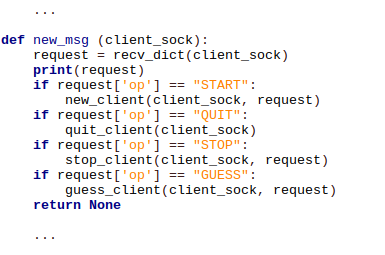
\includegraphics[scale=0.65]{new_msg}   
        \caption{Função chamada sempre que o servidor recebe uma nova mensagem do cliente.}
\end{figure}
Seguidamente o jogador terá que introduzir uma das seguintes operações na linha de comandos: GUESS, STOP ou QUIT.
A tarefa desta função é identificar qual a operação requisitada pelo cliente e encaminhá-la para a função que irá processar e responder ao pedido.
Caso seja feito um pedido de uma operação fora do alcançe da aplicação não ocorre qualquer comportamento por parte do servidor.

\begin{figure}[H]
        \centering
        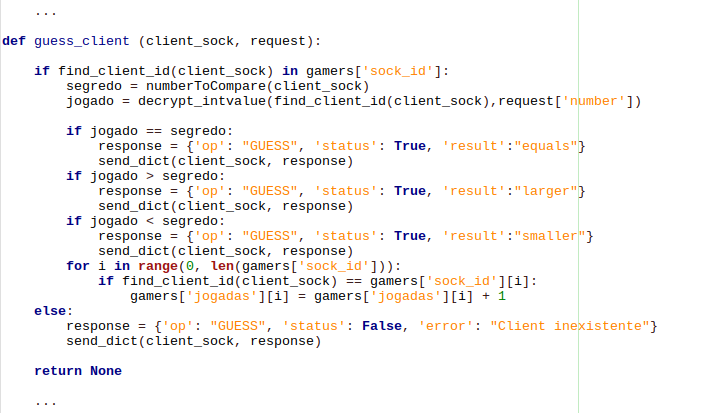
\includegraphics[scale=0.65]{guess_client}      
        \caption{Suporte da jogada de um cliente - Operação GUESS.}
\end{figure}
O utilizador deve introduzir o comando GUESS antes de inserir o seu palpite. No entanto, é essencial averiguar se o cliente que está a jogar tem realmente uma sessão iniciada no jogo.

Se o jogador estiver presente no dicionário "gamers" prosseguimos com o GUESS.Caso contrário, o servidor envia uma mensagem ao cliente com o status: False; e uma mensagem de erro a indicar que este não se encontra na lista de jogadores ativos.

Consideremos agora o caso em que o cliente tem um jogo iniciado. Primeiro, procuramos o valor do número secreto deste cliente através da função "numberToCompare()", que será armazenado na variável segredo. 
\begin{figure}[H]
        \centering
        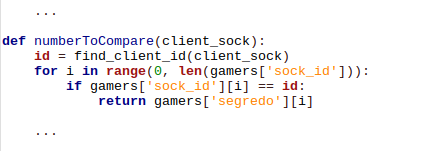
\includegraphics[scale=0.65]{numberToCompare}   
        \caption{Função que devolve o número secreto.}
\end{figure}

Depois, descriptografamos o número inserido pelo jogador(que é passado na mensagem enviada do cliente ao servidor e que depois é encaminhada para a função pelo parâmetro "request") que é armazenado na variável "jogado".
\begin{itemize}
\item Se o número for igual ao número secreto, o servidor envia uma mensagem ao cliente com status: True e result: "equals", a indicar que o jogador acertou no número;
\item Se o número for maior que o segredo, o servidor envia uma mensagem ao cliente com status: True e result: "larger" a indicar que o jogador introduziu um número superior ao número secreto;
\item Se o número for menor que o segredo, o servidor envia uma mensagem ao cliente com status: True e result: "smaller", a indicar que o jogador introduziu um número mais pequeno que o número secreto;
\end{itemize}
Por fim, atualiza no dicionário "gamers" o número de jogadas efetuadas.

\begin{figure}[H]
        \centering
        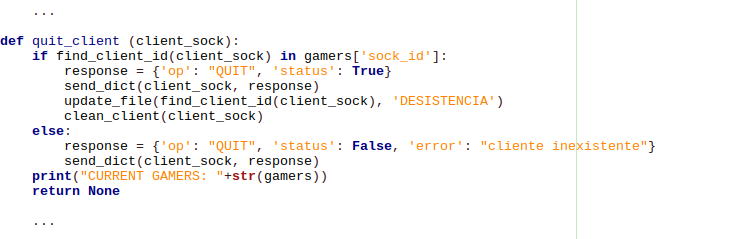
\includegraphics[scale=0.65]{quit_client}       
        \caption{Função chamada quando o cliente pretende desistir do jogo.}
\end{figure}
Caso o jogador queira desistir do jogo, o servidor recebe uma mensagem com o comando QUIT.Isto induz  a função "quit\_client" a conferir se o cliente que pretende desistir encontra-se realmente em jogo. Para isto, verifica se o ID do socket está presente no dicionário "gamers".

Em caso afirmativo, o servidor envia uma mensagem ao cliente com status: True; e atualiza o ficheiro report.csv(recorrendo à função update\_file()) com o resultado "DESISTENCIA". Este resultado indica que a partida foi terminada antes de o jogador adivinhar o número secreto ou antes de atingir o limite de jogadas. Por fim, remove o cliente da lista de jogadores ativos recorrendo à função clean\_client.

Caso contrário, envia uma mensagem ao cliente com status: False; e uma mensagem de erro que explicita o facto de o cliente não ter sido encontrado entre os jogadores ativos.

\begin{figure}[H]
        \centering
        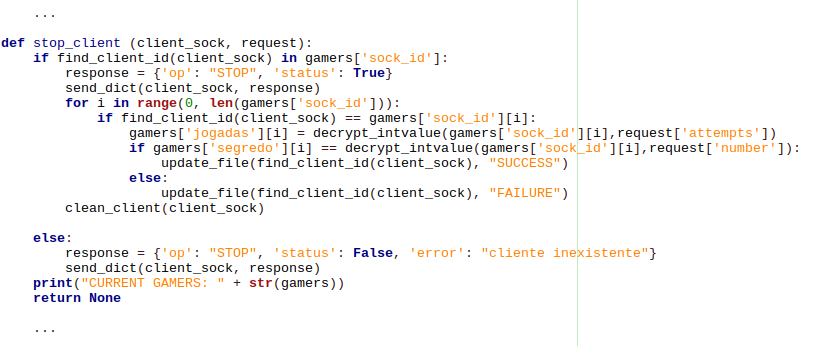
\includegraphics[scale=0.65]{stop_client}       
        \caption{Função responsável por encerrar o jogo.}
\end{figure}
Quando um jogo é terminado ou porque o jogador acertou no número secreto ou porque efetou mais jogadas dos que as que possuía é executada a função "stop\_client".

Para que um jogo seja encerrado, o cliente precisa estar na lista de jogadores ativos, ou seja, no dicionário "gamers".
Se o cliente não se encontrar ativo no jogo, a função envia-lhe uma mensagem com status: False e uma mensagem de erro a indicar que o cliente não se encontra na lista de jogadores ativos.
Caso o cliente esteja ativo no jogo, o servidor envia-lhe uma mensagem com status: True, a indicar que a finalização do jogo foi processada.

O processamento da finalização do jogo dá-se da seguinte forma: 
\begin{enumerate}
\item O servidor atualiza no dicionário "gamers" o número de jogadas efetuadas pelo jogador. Para isso, deve descriptografar o número inteiro enviado pelo cliente com auxílio da função "decrypt\_intvalue()";
\item O servidor verifica se o último número jogado pelo utilizador(que também deve ser descriptografado) coincide com o número secreto.
Em caso afirmativo, atualiza o ficheiro report.csv com os dados do cliente e o resultado final "SUCCESS". Caso contrário, atualiza o ficheiro report.csv com os dados do cliente e o resultado final "FAILURE";
\item Elimina o cliente da lista de jogadores ativos através da função "clean\_client()".

\begin{figure}[H]
        \centering
        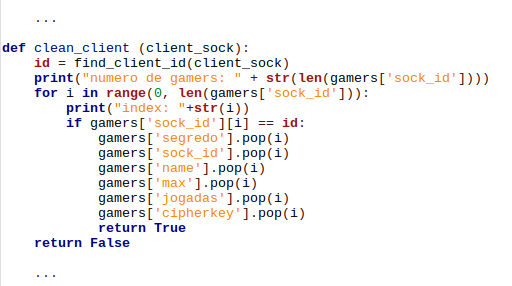
\includegraphics[scale=0.65]{clean_client}      
        \caption{Função chamada sempre que é necessário apagar um jogador da lista de jogadores ativos.}
\end{figure}
Esta função é executada sempre que for necessário excluir um cliente do dicionário "gamers". Isto ocorre quando o cliente se desconecta do servidor, quando termina o jogo ou quando desiste.
A função procura pelo cliente no dicionário "gamers" e caso o encontre, exclui todos os dados a ele associados através do seu respetivo índice.
\end{enumerate}

\subsection{Segurança}
\subsubsection{Encriptação}
\begin{figure}[H]
        \centering
        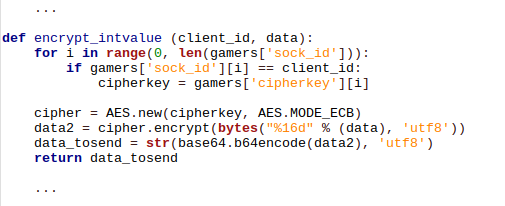
\includegraphics[scale=0.65]{encrypt_intvalue}  
        \caption{Função para encriptar valores a enviar em formato JSON com codificação base64.}
\end{figure}

Cada número inteiro comunicado entre o servidor e o cliente é encriptado por blocos usando a função AES-128 no modo ECB. A encriptação é realizada do seguinte modo: 
\begin{enumerate}
\item Identificação da chave de cifragem relativa ao cliente atual comparando o ID passado como argumento da função e os IDs presentes no dicionário "gamers";
\item Conversão do inteiro numa string binária de 128 bits;
\item Codificação da string no formato Base64 com o intuito dos criptogramas serem suportados pelo JSON;
\item Devolução pela função do valor codificado e encriptado para que possa ser enviado. 
\end{enumerate}
\subsubsection{Descriptação}
\begin{figure}[H]
        \centering
        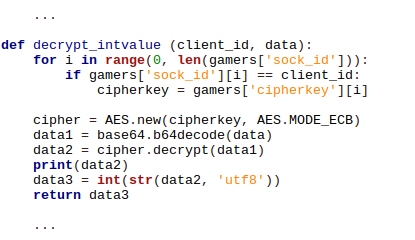
\includegraphics[scale=0.65]{decrypt_intvalue}  
        \caption{Função para desencriptar valores recebidos em formato json com codificação base64.}
\end{figure}
Cada número inteiro comunicado entre o servidor e o cliente é descriptado por blocos usando a função AES-128 em modo ECB. A descriptação ocorre do seguinte modo:
\begin{enumerate}
\item Identificação da chave de cifragem relativa ao cliente atual comparando o ID passado como argumento da função e os IDs presentes no dicionário "gamers";
\item Descodificação dos dados passados à função como argumento no formato Base64 e descriptação do seu conteúdo;
\item Codificação para um valor inteiro;
\item Devolução do valor inteiro pela função.
\end{enumerate}

\subsection{Main}
\begin{figure}[H]
        \centering
        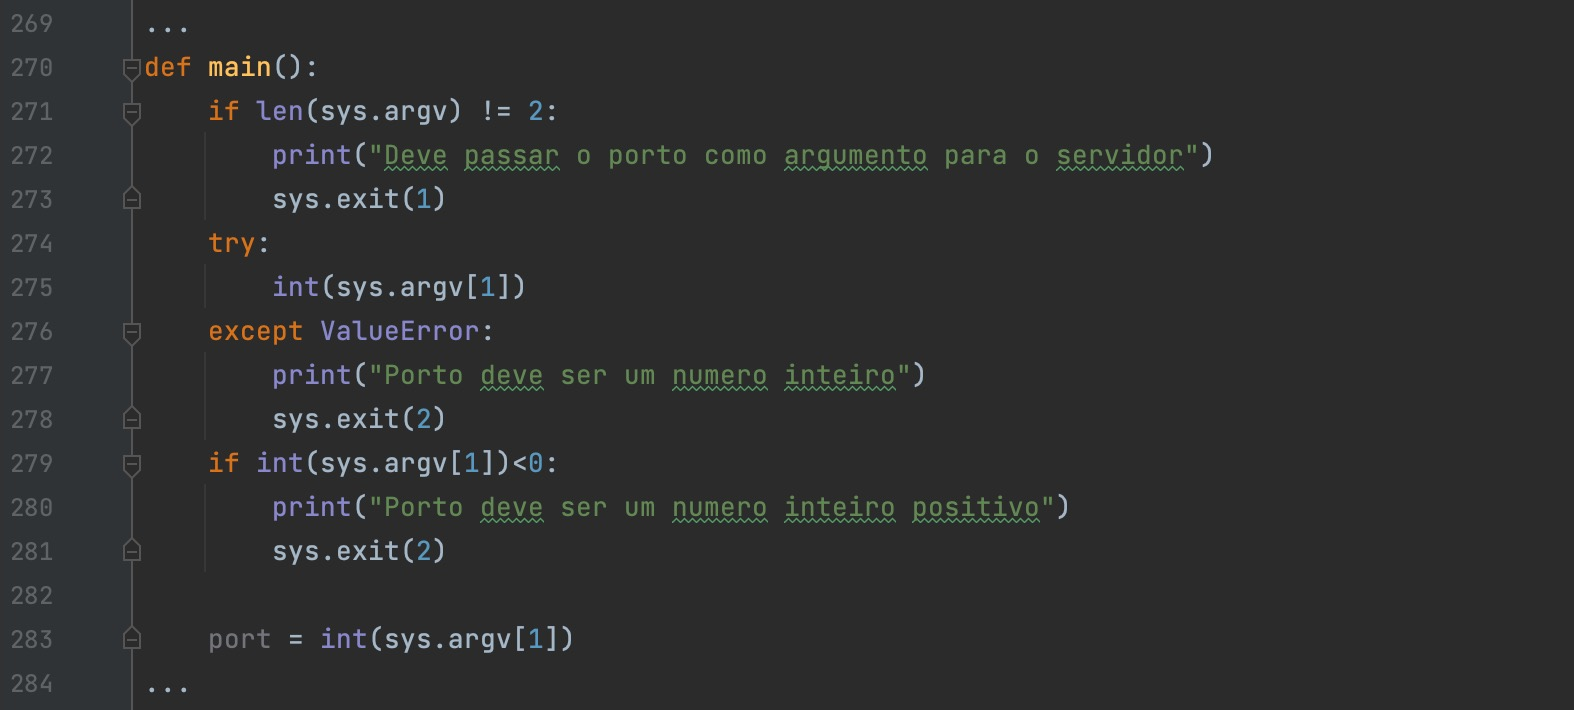
\includegraphics[scale=0.20]{serverMain}      
        \caption{Função que permite o funcionamento correto de todo o servidor.}
\end{figure}

Esta função permite:
\begin{itemize}
\item Nas linhas 271-273 verificar se o servidor é iniciado com um argumento(porto). Caso não seja, o programa encerra com uma mensagem de erro;
\item Nas linhas 274-281 verificar se o porto é um número inteiro. Se não for, o programa é encerrado com uma mensagem de erro;
\item Na linha 283 é atribuído o valor do porto à variável.
\end{itemize}

\section{Cliente}
O programa cliente consiste em permitir que um utilizador jogue o jogo "Adivinhe o número secreto" ao introduzir as operações START, GUESS,QUIT e o seu palpite na linha de comandos.

O programa cliente é constítuido por uma chave de cifragem e pelas seguintes funções: \textbf{encrypt\_intvalue}, \textbf{decrypt\_intvalue}, \textbf{validate\_response}, \textbf{quit\_action}, \textbf{run\_client} e \textbf{main}.
\subsection{Funcionamento geral do jogo}
Para que a aplicação funcione corretamente é essencial que exista uma função no programa cliente que valide a resposta enviada pelo servidor. Para isso é executada a função "validate\_response".
\begin{figure}[H]
        \centering
        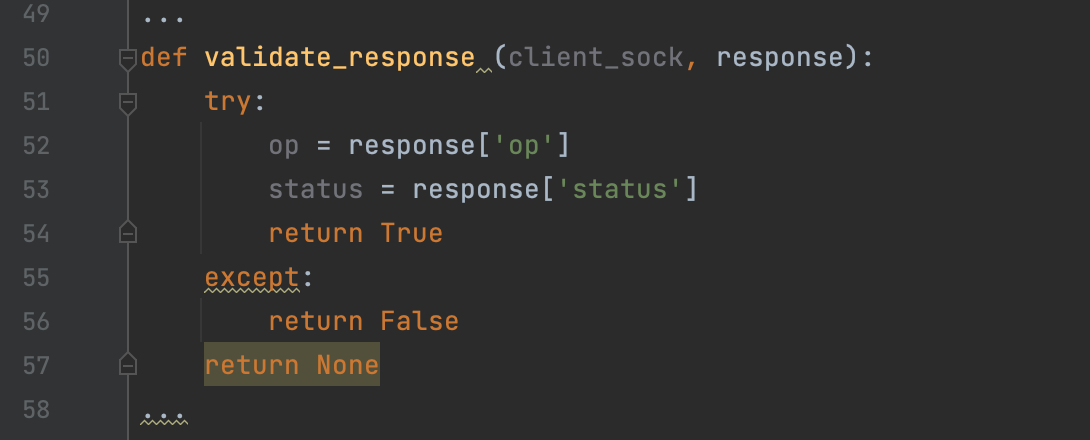
\includegraphics[scale=0.43]{validateResponse}      
        \caption{Função que valida a resposta do servidor recebida pelo cliente.}
\end{figure}
A resposta do servidor é válida quando é do tipo " 'op' : xxxx, 'status' : xxxx".Assim, usa-se um "try-catch" que tenta aceder aos valores de 'op' e 'status'. Se o acesso for possível é devolvido "True". Caso o acesso falhe é retornado "False".

A função que gerencia o programa cliente é a função "run\_client".
\begin{figure}[H]
        \centering
        \includegraphics[scale=0.43]{runclient1}      
        \caption{Variáveis da função \textbf{run\_client}}
\end{figure}
As variáveis da função "run\_client" desempenham as seguintes funcionalidades: 
\begin{itemize}
\item emUso: Enquanto estiver True, o programa irá estar à espera de novos comandos. A função STOP pode encerrar o ciclo ao mudar esta variável para False;
\item jogadas: Número de jogadas efetuadas pelo jogador;
\item jogMax: Número máximo de jogadas que um jogador pode fazer. É uma variável vazia até que receba o número de tentativas enviadas pelo servidor após a introdução do comando START pelo cliente;
\item auto: Os comandos START, GUESS e QUIT devem ser introduzidos pelo utilizador. O comando STOP é inserido automaticamente pelo sistema quando é detectado o fim de um jogo. Assim, quando esta variável for TRUE, o próximo comando a ser executado será feito automaticamente pelo sistema e quando for FALSE, o programa fica à espera de um input do utilizador;
\item nextCom: Próximo comando a ser executado em modo automático;
\item lastAttempt: Último número jogado pelo utilizador ao executar o comando GUESS.
\end{itemize}

\begin{figure}[H]
        \centering
        \includegraphics[scale=0.43]{runclient2}      
        \caption{Função \textbf{run\_client}}
\end{figure}
Neste ciclo while o programa está à espera de novos comandos a serem introduzidos pelo cliente(emuso == True).Logo, se auto == False o próximo comando a ser executado deverá ser introduzido pelo utilizador. Caso contrário, o comando executado será "nextCom".

\begin{figure}[H]
        \centering
        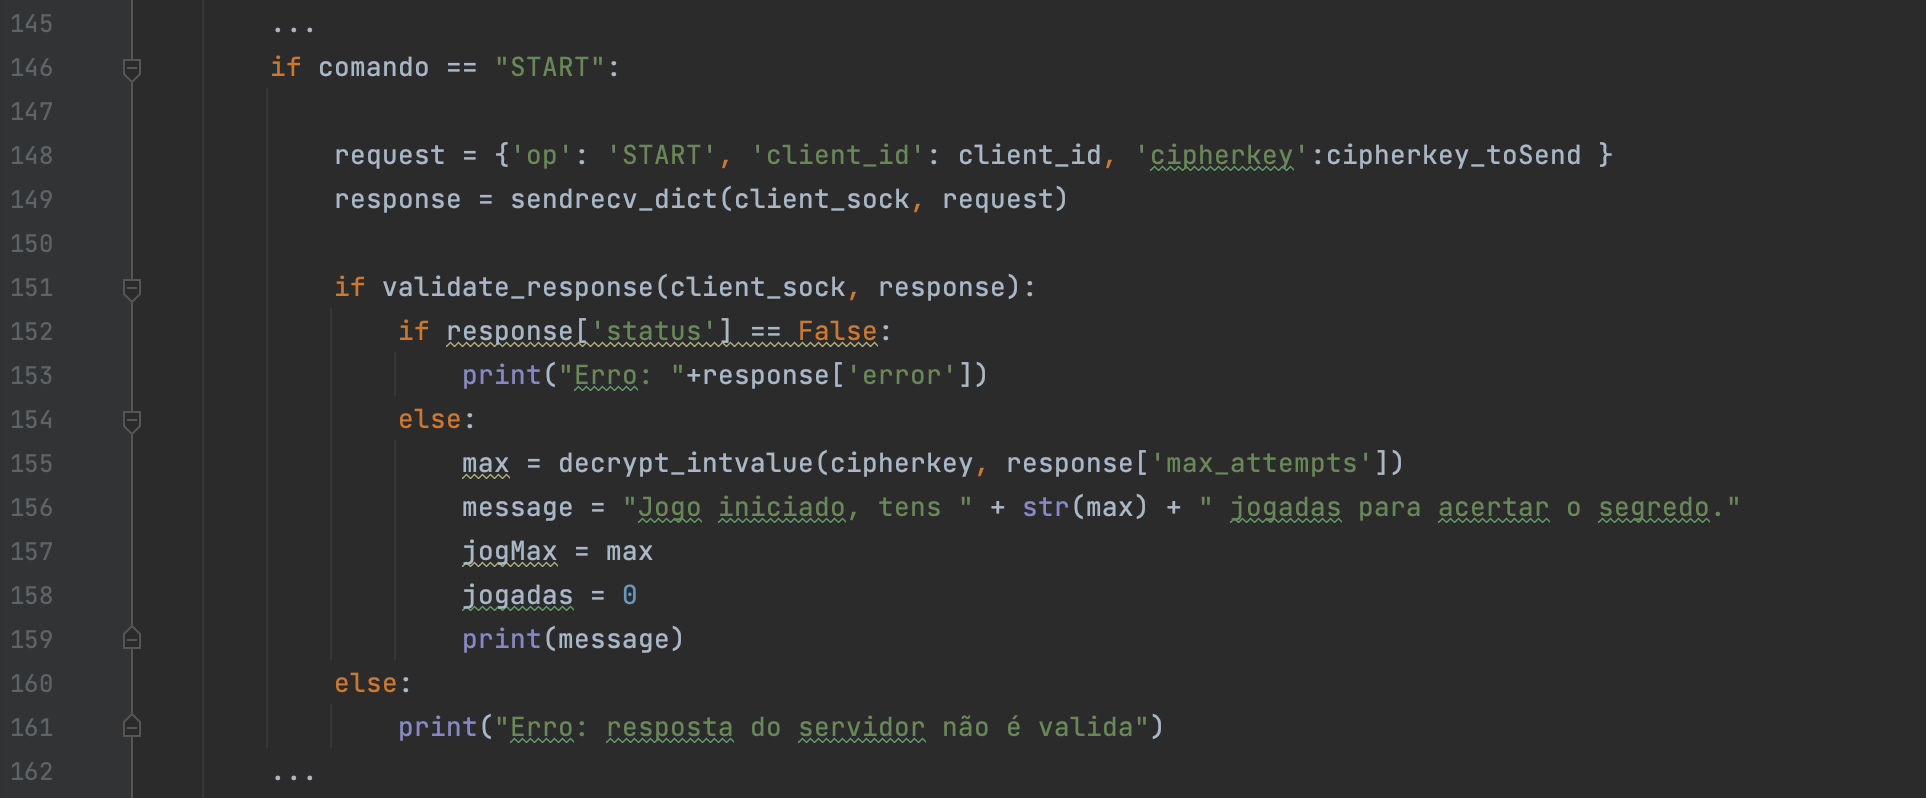
\includegraphics[scale=0.43]{start}      
        \caption{Caso em que é inserido o comando START.}
\end{figure}
Por outro lado, se for introduzido o comando START, o cliente envia uma mensagem ao servidor indicando a operação que deseja executar, o id do cliente(inserido na linha de comandos ao executar o programa), e a chave de cifra codificada. Ao receber uma resposta, esta será validada pela função "validate\_response" e caso seja válida: 
\begin{enumerate}
\item Verifica o status da resposta. Se for False, deverá imprimir uma mensagem de erro recebida do servidor. Se for True irá descriptografar o número máximo de jogadas para esta partida recorrendo à função "decrypt\_intvalue";
\item Inicia a contagem de jogadas, atribuindo o valor zero à variável "jogadas";
\item Mostra uma mensagem de confirmação ao utilizador.
\end{enumerate}
Se a resposta do servidor não for válida:
\begin{enumerate}
\item Mostra uma mensagem de erro referente ao erro identificado pelo servidor.
\end{enumerate}

\begin{figure}[H]
        \centering
        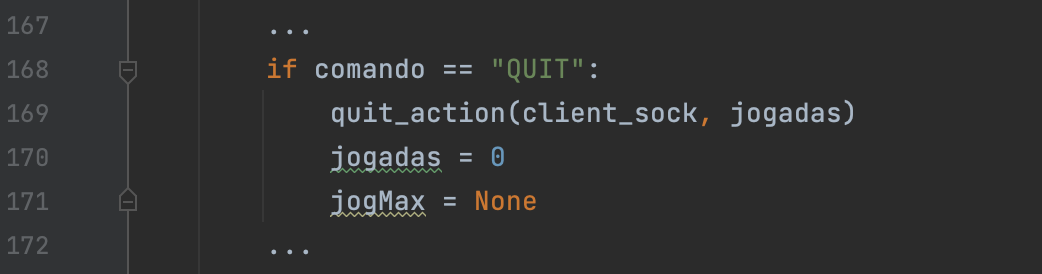
\includegraphics[scale=0.43]{quit}      
        \caption{Caso em que é inserido o comando QUIT.}
\end{figure}
Se o comando introduzido for o QUIT, o programa processa o pedido do cliente recorrendo à função "quit\_action()" e as variáveis "jogadas" e "jogMax" voltam aos seus estados iniciais.
\begin{figure}[H]
        \centering
        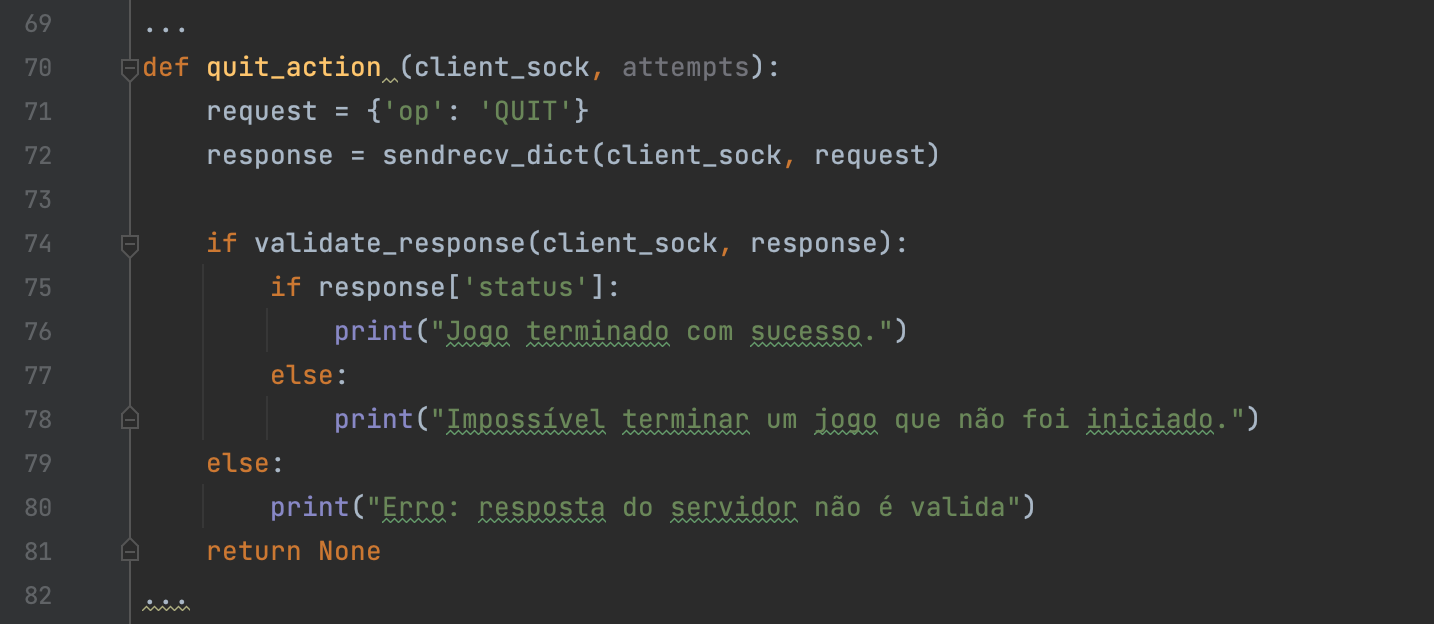
\includegraphics[scale=0.43]{quitAction}      
        \caption{Função \textbf{quit\_action}.}
\end{figure}
A função \textbf{quit\_action} processa a operação QUIT. Quando o utilizador introduzir o comando QUIT no terminal esta função irá enviar uma mensagem ao servidor e aguardar por uma resposta.Esta resposta é devolvida pela função "sendrecv\_dict()".

Depois, a função \textbf{quit\_action} armazena a resposta na variável "response".Seguidamente, recorrendo à função "validate\_response" verifica se a resposta é válida. Em caso afirmativo verifica o 'status' da resposta. Se o status for TRUE o jogo foi terminado com sucesso(imprime uma mensagem de sucesso). Se o status for False, indica que o servidor não encontrou o cliente atual na lista de jogadores ativos e imprime uma mensagem de erro.Caso a resposta do servidor não seja válida, é imprimida uma mensagem de erro correspondente.

\begin{figure}[H]
        \centering
        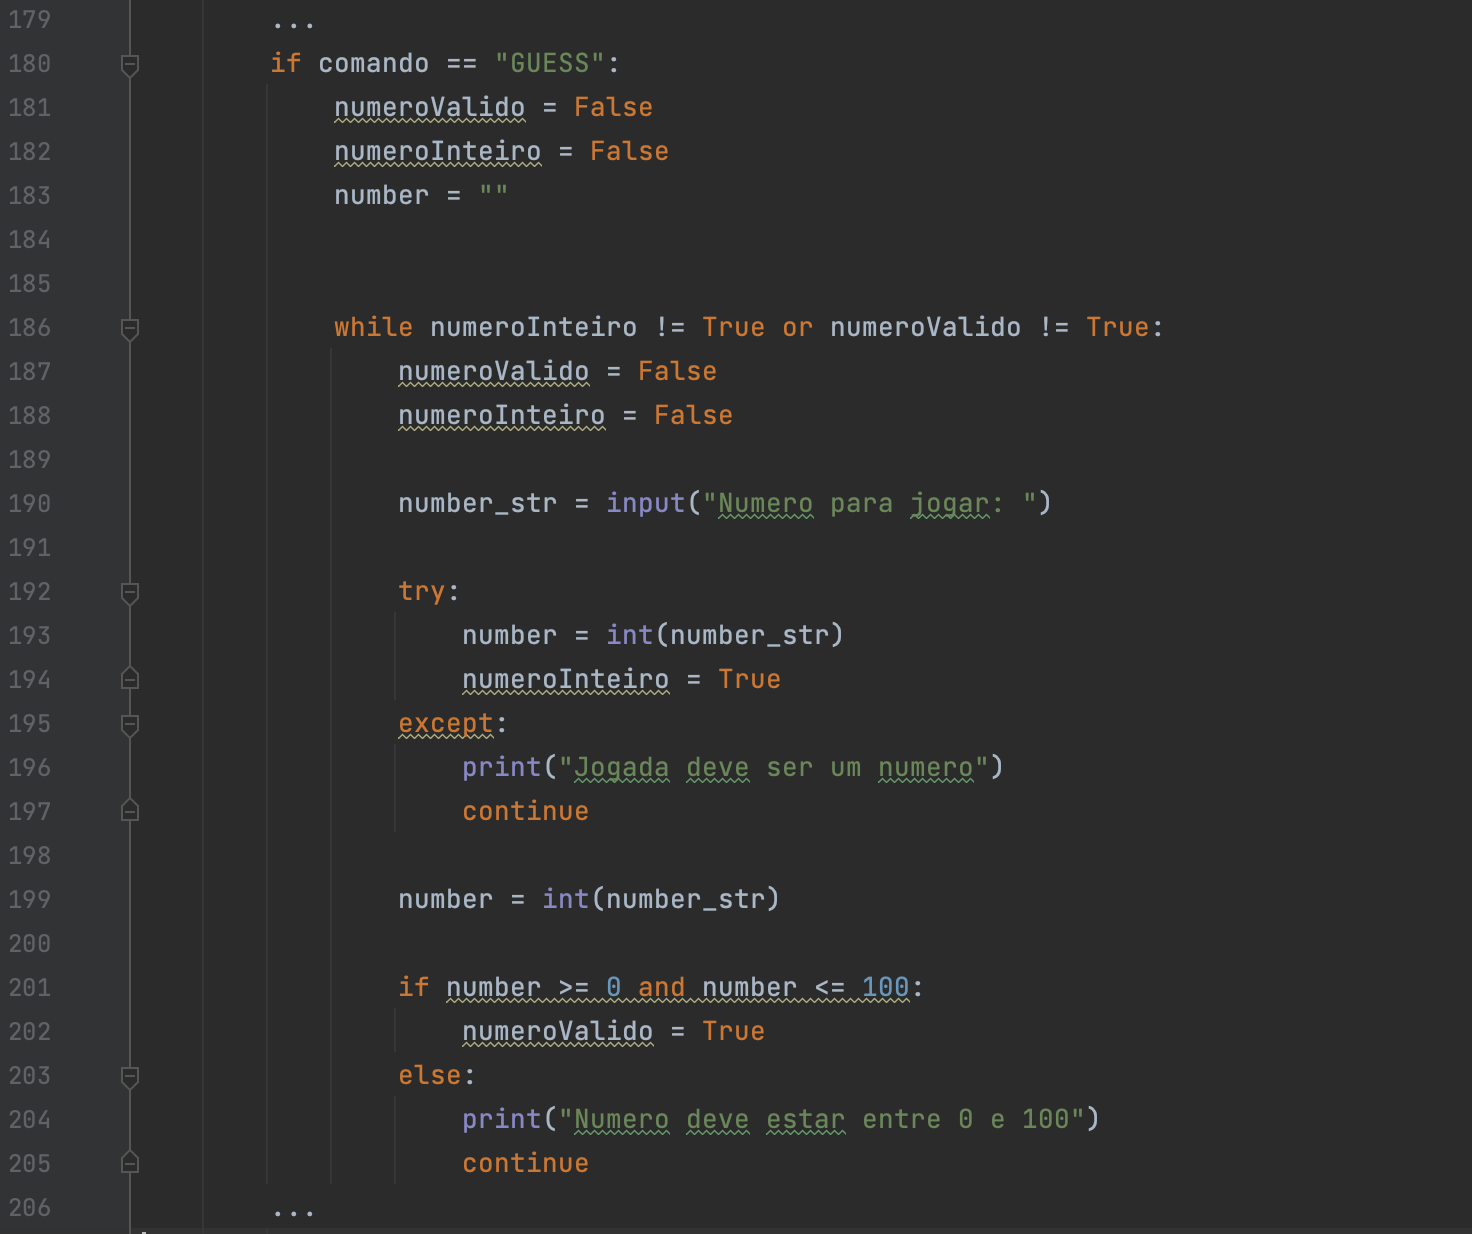
\includegraphics[scale=0.43]{guess1}      
        \caption{Caso em que é inserido o comando GUESS.}
\end{figure}
Se o comando introduzido for GUESS, têm que ser inicializadas duas novas variáveis para verificar se o número introduzido pelo utilizador é de facto um número inteiro e se é válido(se está entre 0 e 100).
Nas linhas 186-205 é verificado se o valor introduzido é um inteiro válido e se não for, o programa pede um novo valor ao utilizador.
\begin{figure}[H]
        \centering
        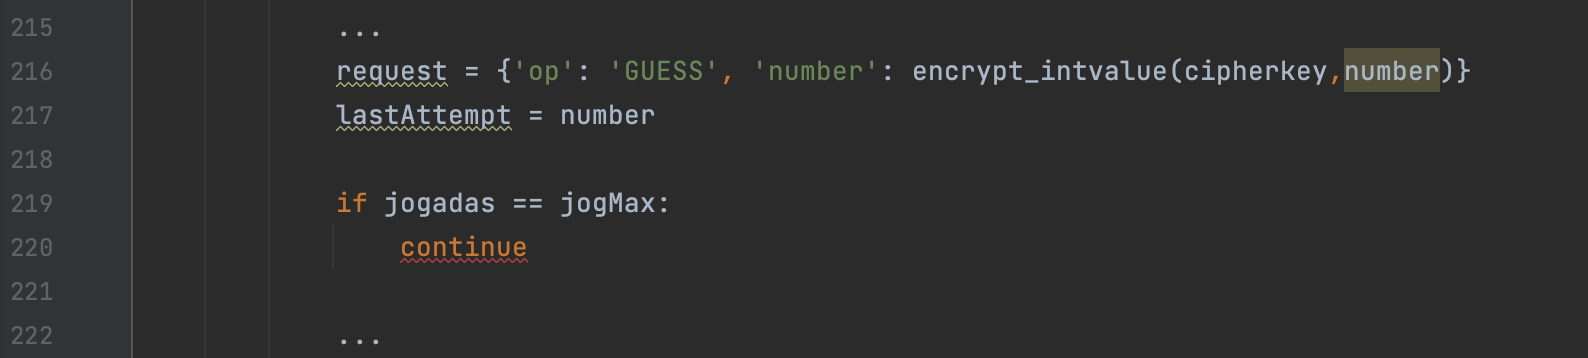
\includegraphics[scale=0.43]{guess2}      
        \caption{Caso em que é inserido o comando GUESS.}
\end{figure}
Tendo já a certeza de que o palpite introduzido pelo cliente é um número inteiro válido prepara-se a mensagem que será enviada ao servidor. A mensagem contém o número jogado após ser criptografado recorrendo à função "encrypt\_intvalue()".

Na linha 217 a variável "lastAttempt" recebe o número que foi jogado.
Na linha 219 é verificado se o número de jogadas é igual ao número máximo de jogadas. Se sim, nada ocorre e o ciclo passa para a próxima execução.

\begin{figure}[H]
        \centering
        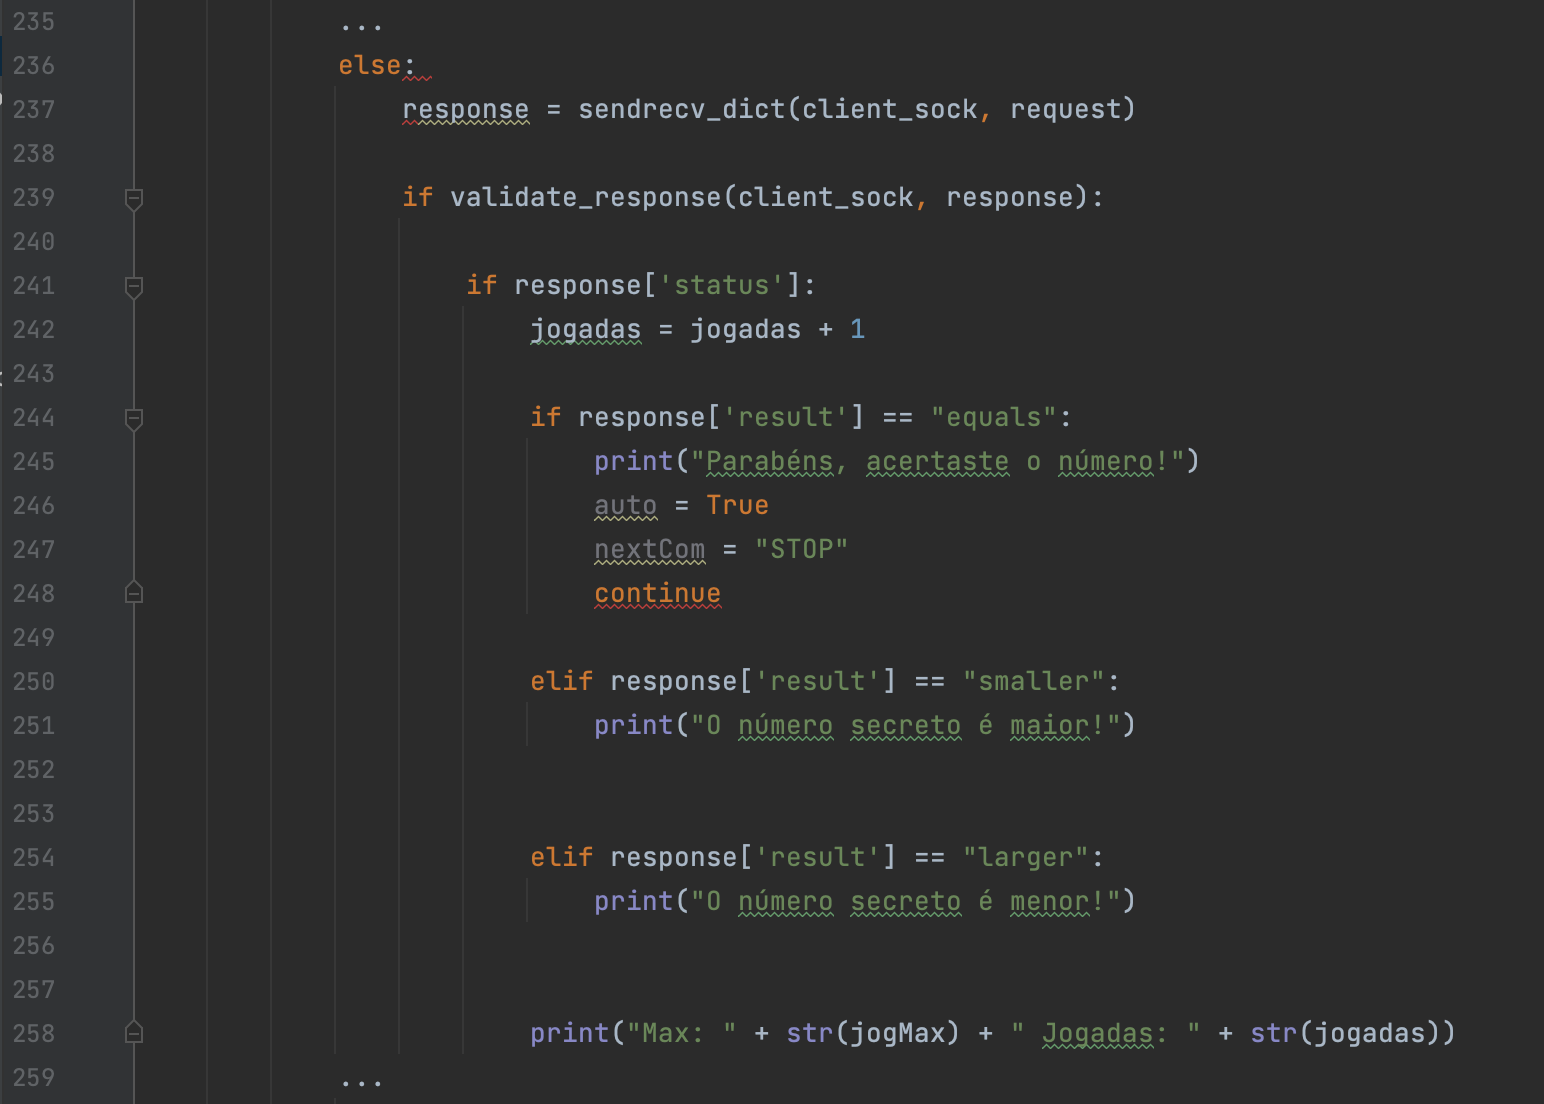
\includegraphics[scale=0.43]{guess3}      
        \caption{Caso em que é inserido o comando GUESS.}
\end{figure}
Caso o jogador ainda tenha jogadas disponíveis a mensagem é enviada ao servidor e a sua resposta é validada pela função "validate\_response()".
Nas linhas 241-242 verificamos que se a resposta for válida e se o status for True, ou seja, se o servidor não reportar erros, a resposta é processada sendo somado 1 ao número de jogadas. De seguida, é avaliado o resultado reportado pelo servidor.

Se o resultado for "equals", vemos pelas linhas 244-248, que o jogador acertou no número. E, portanto é atribuído True à variável "auto" e STOP à "nextCom" ficando implícito que o jogo acabou e que o comando STOP será executado automaticamente na próxima execução do ciclo while.

Nas linhas 250-251 é retratado que se o resultado for "smaller" é exibida uma mensagem "O número secreto é maior!".E, nas linhas 254-255 é imprimida uma mensagem "O número secreto é menor!" quando o resultado for "larger".

No fim de cada tentativa é relembrado ao jogador o número máximo de jogadas que pode fazer e o número de jogadas que já efetuou - linha 258.

\begin{figure}[H]
        \centering
        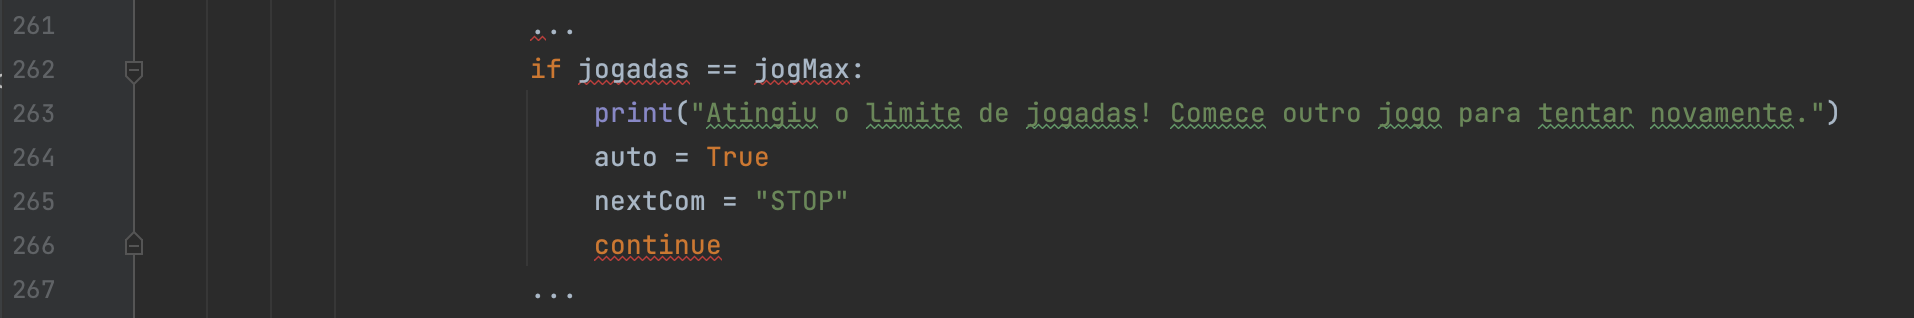
\includegraphics[scale=0.43]{guess4}      
        \caption{Caso em que é inserido o comando GUESS.}
\end{figure}

Se o número de jogadas efetuadas for igual ao número máximo de jogadas, é mostrada uma mensagem "Atingiu o limite de jogadas!Comece outro jogo para tentar novamente" e é atribuído True à variável "auto" e STOP à variável "nextCom".

\begin{figure}[H]
        \centering
        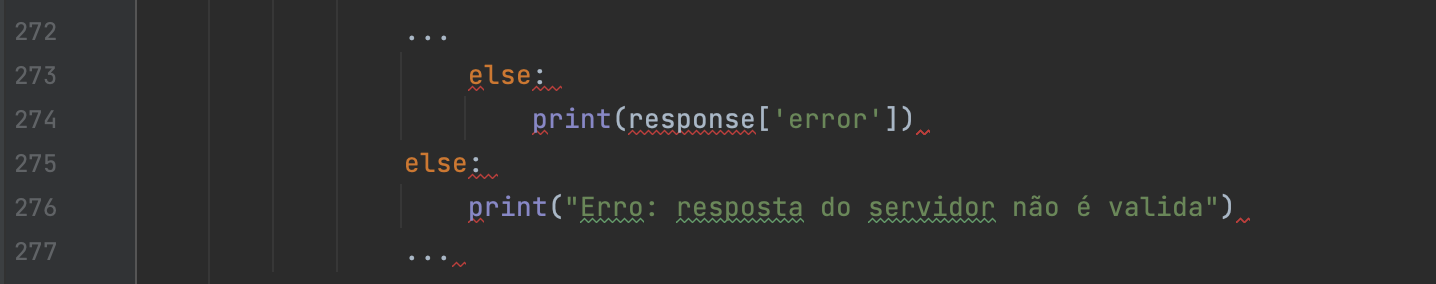
\includegraphics[scale=0.43]{guess5}      
        \caption{Caso em que é inserido o comando GUESS.}
\end{figure}
Se o status da mensagem recebida do servidor for False, é exibida uma mensagem contendo o erro reportado ao servidor - linhas 273-274.
Se a resposta do servidor não for válida, é mostrada a respetiva mensagem de erro - linhas 275-276.

\begin{figure}[H]
        \centering
        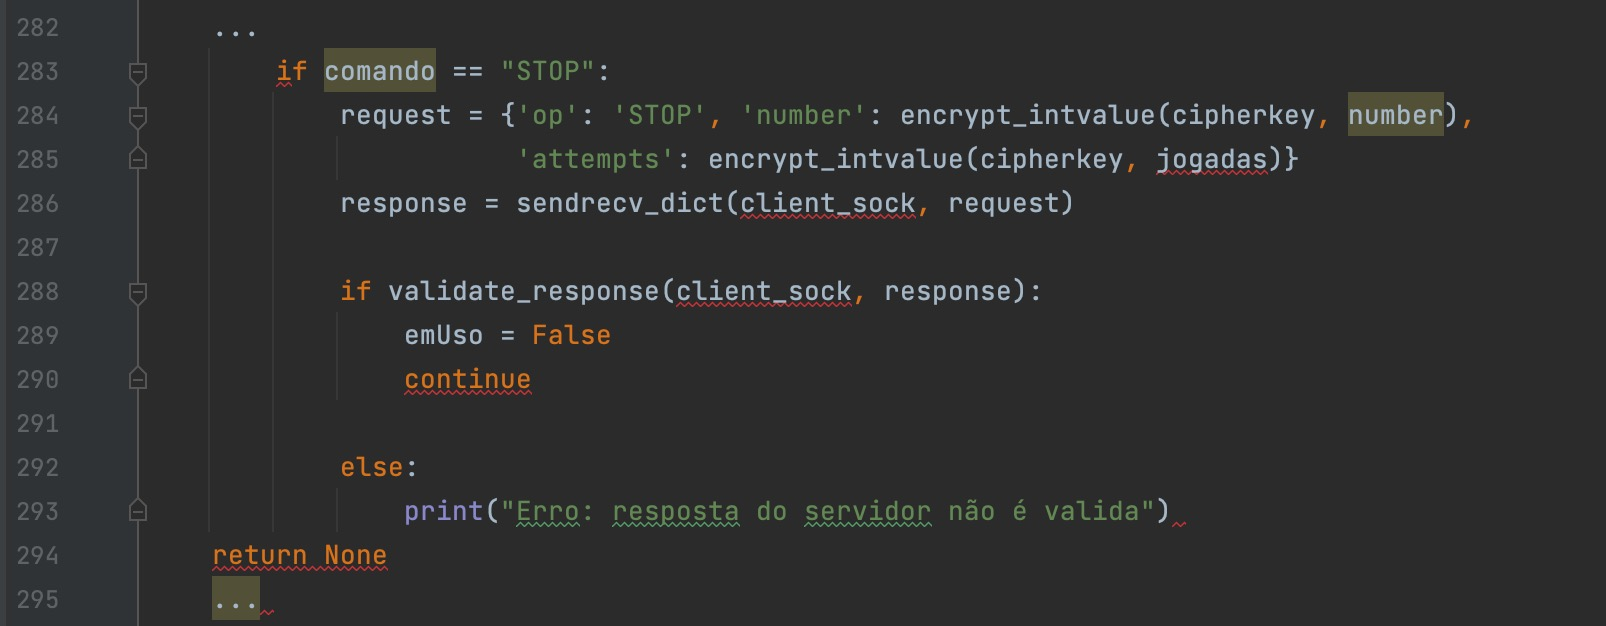
\includegraphics[scale=0.20]{stop}      
        \caption{Caso em que é inserido o comando STOP.}
\end{figure}

Se o comando executado for o comando STOP, é enviada uma mensagem que será posteriormente enviada ao servidor com o valor criptografado do último número jogado e do número total de jogadas(recorrendo à função "encrypt\_intvalue()").
Nas linhas 287-289 o jogo é terminado com sucesso se a resposta do servidor for válida e é atribuída  à variável "emUso" o valor False.
Caso a resposta do servidor não seja válida, é exibida a respetiva mensagem de erro - linhas 291-292.


\subsection{Segurança}
\subsubsection{Encriptação}
\begin{figure}[H]
        \centering
        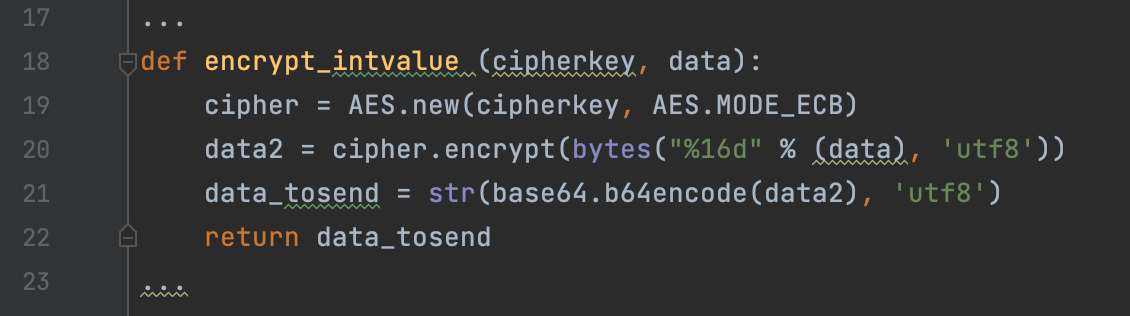
\includegraphics[scale=0.40]{encrypt}      
        \caption{Função para encriptar valores a enviar em formato JSON com codificação base64.}
\end{figure}
Cada número inteiro comunicado entre o servidor e o cliente é encriptado por blocos usando a função AES-128 no modo ECB. A encriptação é realizada do seguinte modo: 
\begin{enumerate}
\item Conversão do inteiro numa string binária de 128 bits já que a chave de cifragem é passada como argumento da função.
\begin{figure}[H]
        \centering
        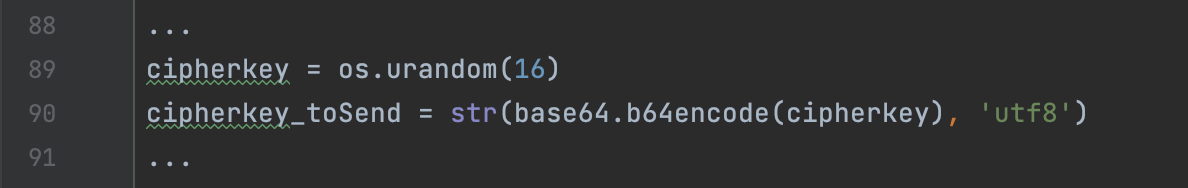
\includegraphics[scale=0.40]{chaveCifra}      
        \caption{Chave de cifragem gerada e codificada no modelo Base64 para ser enviada ao servidor.}
\end{figure}
\item Codificação no formato Base64 para que os criptogramas sejam suportados pelo JSON;
\item A função "encrypt\_intvalue" devolve o valor que foi codificado e encriptado para que possa ser enviado para o servidor.
\end{enumerate}
\subsubsection{Descriptação}
\begin{figure}[H]
        \centering
        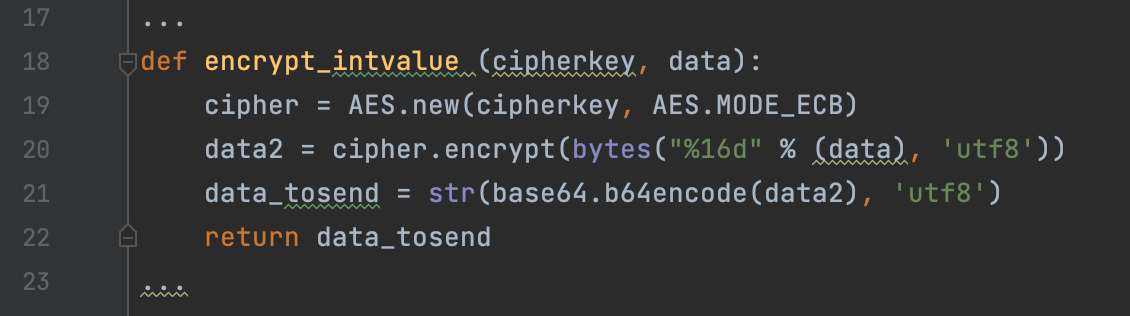
\includegraphics[scale=0.40]{encrypt}      
        \caption{Função para desencriptar valores recebidos em formato JSON com codificação base64.}
\end{figure}

Cada número inteiro comunicado entre o servidor e o cliente é descriptado por blocos usando a função AES-128 em modo ECB. A descriptação ocorre do seguinte modo:
\begin{enumerate}
\item Descodificação dos dados passados à função "decrypt\_intvalue" como argumento no formato Base 64 já que a chave de cifragem é passada como argumento da função;
\begin{figure}[H]
        \centering
        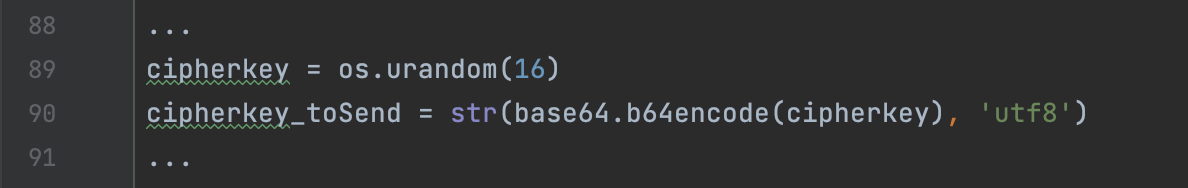
\includegraphics[scale=0.40]{chaveCifra}      
        \caption{Chave de cifragem gerada e codificada no modelo Base64 para ser enviada ao servidor.}
\end{figure}
\item Descriptação do conteúdo dos dados;
\item Codificação num valor inteiro e a sua devolução por parte da função.
\end{enumerate}
\subsection{Main}
A função main do programa client é responsável por verificar se no momento em que o programa é executado, os argumentos são passados para a linha de comandos de forma correta.
O programa pode ser executado de dois modos:
\begin{itemize}
\item Com três argumentos: ID, Porto e Máquina;
\item Com dois argumentos: ID e Porto.
\end{itemize}
No caso em que a máquina está omitida nos argumentos deve-se considerar a máquina local(127.0.0.1).
A variável "instead2" controla os modos de execução do programa. Quando instead2 == True está a funcionar em modo de dois argumentos com a máquina local automaticamente designada como destino.

Vamos analisar o código desta função:
\begin{figure}[H]
        \centering
        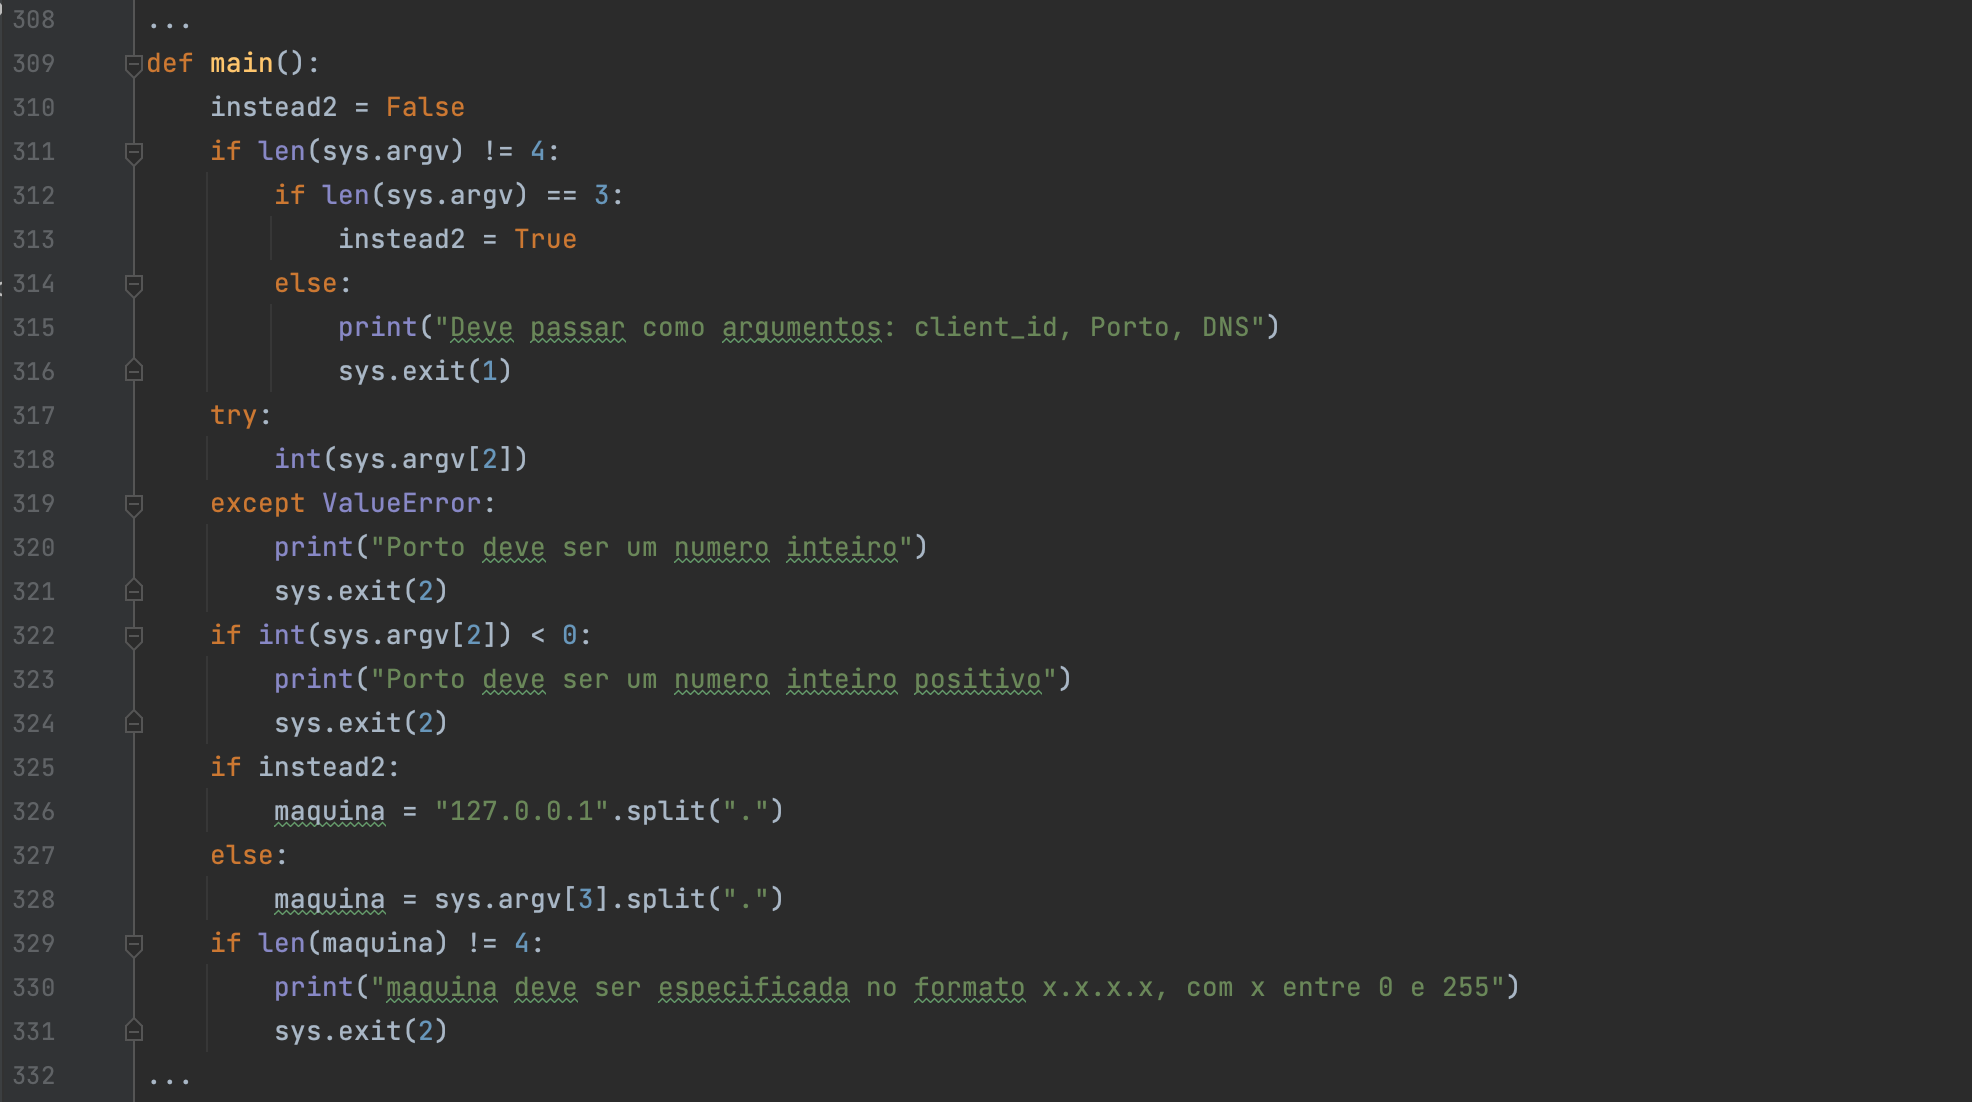
\includegraphics[scale=0.40]{main1}      
        \caption{Função main}
\end{figure}

\begin{itemize}
\item Nas linhas 310-316 é verificado se são passados três argumentos. Se tal não se verificar é verificado se foram passados dois argumentos. Neste caso, "instead" recebe o valor True. Caso contrário, o programa encerra com uma mensagem a especificar como deve ser feita a execução;
\item Nas linhas 317-321 verifica-se se o argumento do Porto é um número inteiro ao tentar converter a sua string para int. Se a conversão falhar, o programa termina com uma mensagem de erro.E, nas linhas 322-324 é averiguado se o argumento do Porto é um número inteiro positivo;
\item De seguida nas linhas 325-328 a máquina designada é a máquina local 127.0.0.1. caso o programa esteja a correr em modo de dois argumentos. Se isto não se verificar, é atribuída à variável o valor passado na linha de comandos e a string da máquina é separada num array de strings para que possam ser analisados os seus elementos separadamente;
\item Nas linhas 329-331 é verificado se o array dos elementos da maquina possui quatro elementos. Se tal não acontecer é encerrado o programa com uma mensagem de erro;
\end{itemize}

\begin{figure}[H]
        \centering
        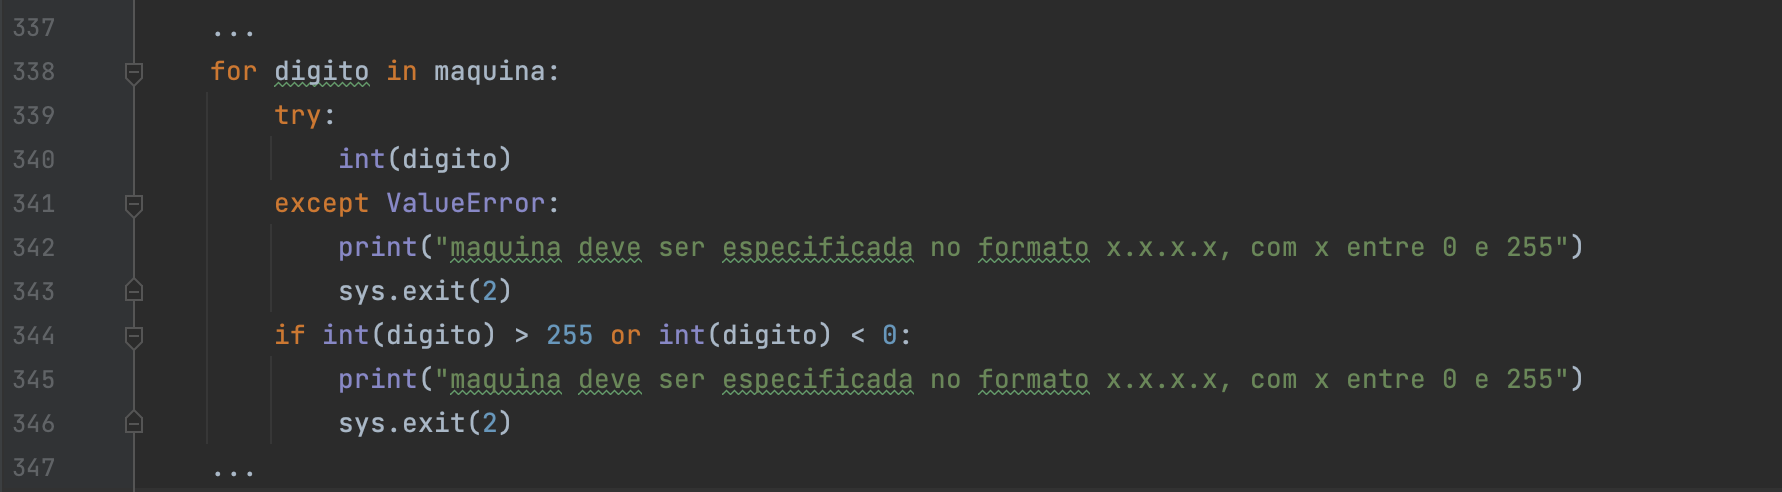
\includegraphics[scale=0.40]{main2}      
        \caption{Função main}
\end{figure}
Aqui é verificado para cada elemento do array se são números inteiros ao tentar fazer a conversão de string para int. Verifica-se também se os elementos estão dentro do intervalo válido, entre 0 e 255. Se algum dos casos não se verificar é reportada uma mensagem de erro.

\begin{figure}[H]
        \centering
        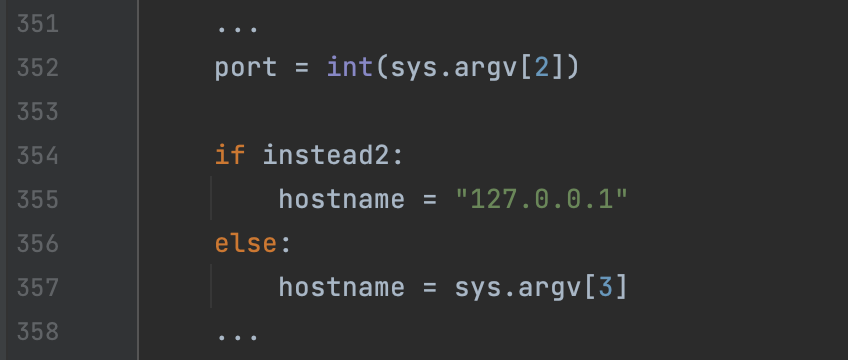
\includegraphics[scale=0.40]{main3}      
        \caption{Função main}
\end{figure}
Por fim, tendo já verificado a validade dos argumentos passados na linha de comandos, são atribuídos às suas respetivas variáveis de acordo com o modo de execução, com dois ou três argumentos.

\section{Testes unitários e funcionais}
\subsection{Testes Funcionais}

Para assegurar que os programas, cliente e servidor, desenvolvidos durante este projeto estão a funcionar corretamente, de acordo com aquilo que é esperado pelos desenvolvedores, implementamos uma série de testes funcionais que se encarregam de verificar a robustez do
código previamente descrito no capítulo de metodologia deste relatório.

A intenção por trás da inclusão dos testes é nos certificarmos de que, quanto à inicialização de ambos os programas com a passagem de argumentos na linha de comandos, o código é capaz de identificar as falhas neste processo, comunicá-las ao utilizador (para que este
possa inserir argumentos corretos na próxima tentativa de execução), e encerrar o programa corretamente, sem maiores impactos negativos que poderiam advir da passagem de argumentos inválidos, ou insuficientes ao sistema.

Para implementar testes funcionais em Python, primeiro instalamos e importamos o pacote ‘pytest’, que suportará o desenvolvimento dos mesmos, em conjunto com os pacotes ‘Popen’ e ‘PIPE’ advindos de ‘subprocess’, num novo ficheiro chamado ‘funcTests.py’.

Dentro deste ficheiro, definimos duas funções, as quais representam os dois macro-cenários de possíveis erros durante a execução inicial dos programas: ‘numArgs()’, que trata de verificar a robustez dos programas quando lidando com argumentos a menos, ou a mais, do que
o esperado para suas respetivas execuções; e ‘invalidArgs()’, que tal como seu nome diz, irá verificar a robustez dos programas quando lidando com argumentos em formatos inválidos, ou seja, diferentes dos esperados pelo sistema ao processá-los.
\begin{figure}[H]
        \centering
        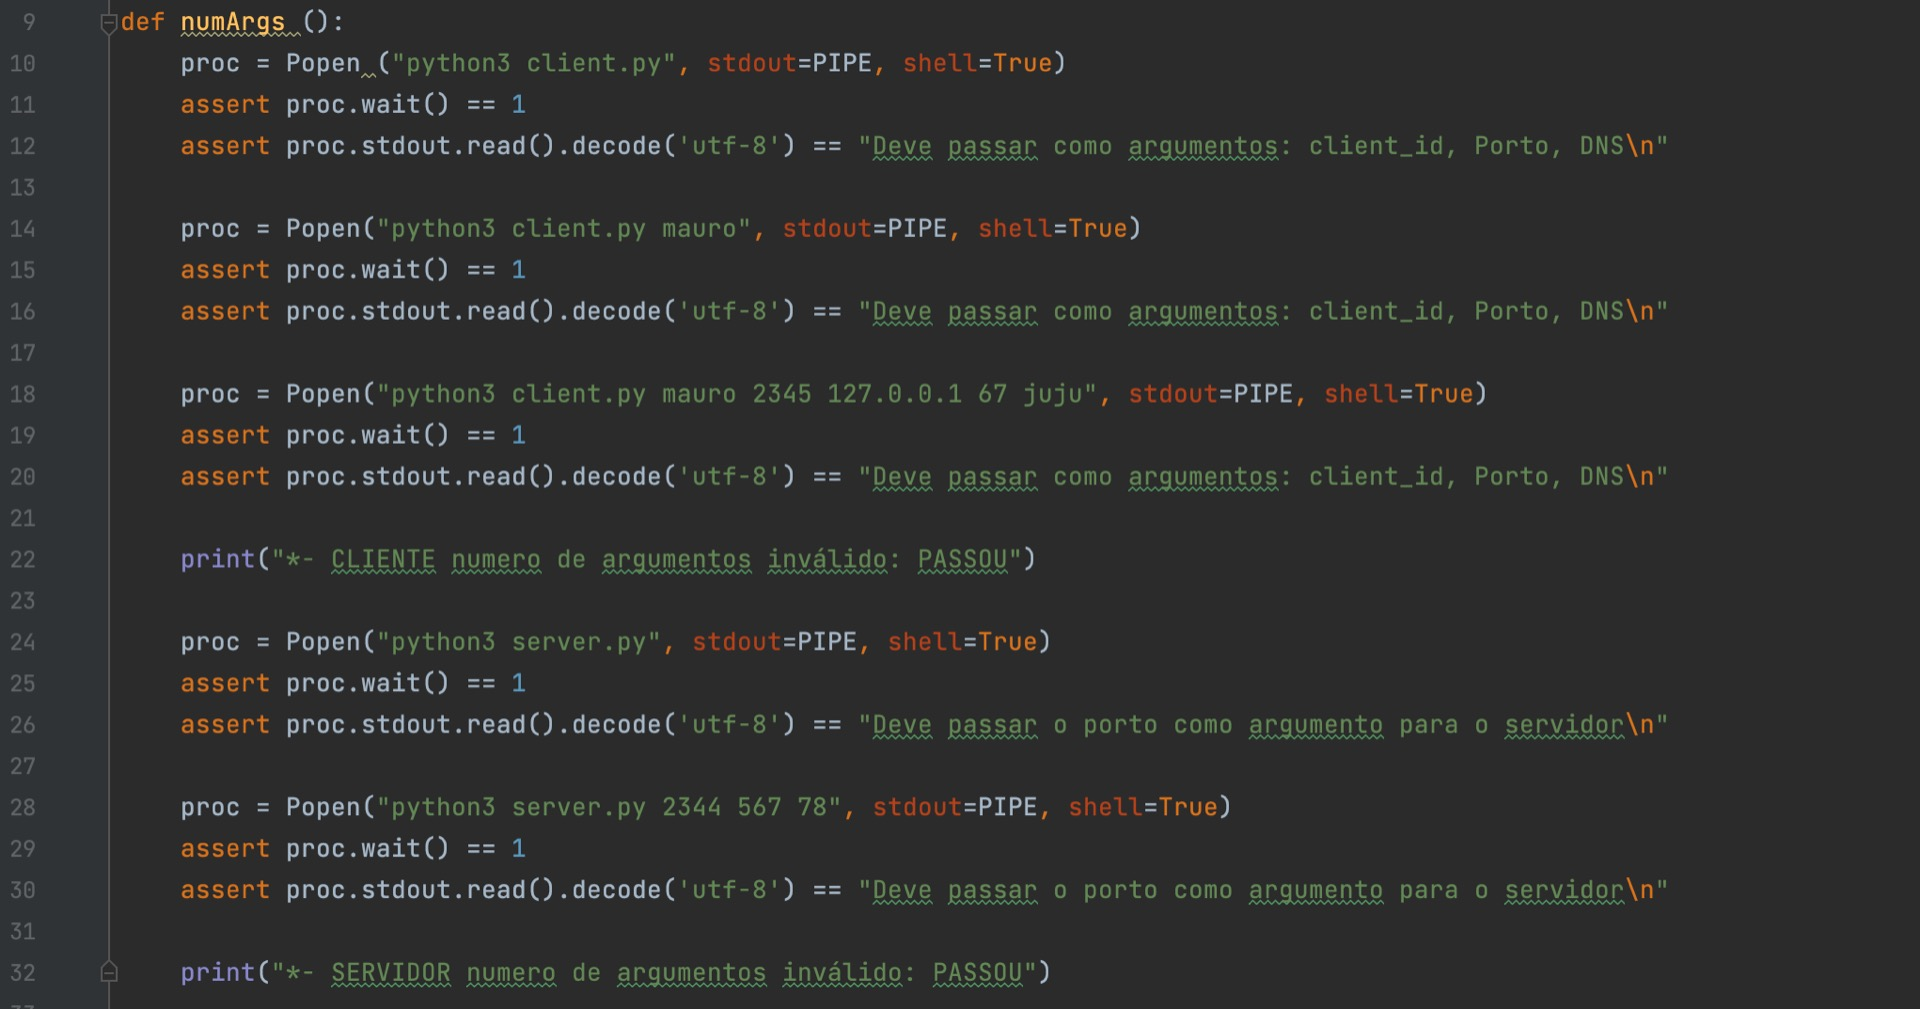
\includegraphics[scale=0.20]{testefuncional}      
\end{figure}
Todos os erros relativos ao número de argumentos inválidos implicam que a execução do programa termine, com código ‘1’. Por isso fazemos uma asserção para cada teste, de que o código retornado por ele deve ser também 1. A segunda asserção também implementada para testes dentro desta função, diz respeito à mensagem que é retornada pelo programa, quando identificada a falha. Caso a mensagem retornada, seja aquela que se esperava, então o programa
lidou corretamente com as falhas.
\begin{figure}[H]
        \centering
        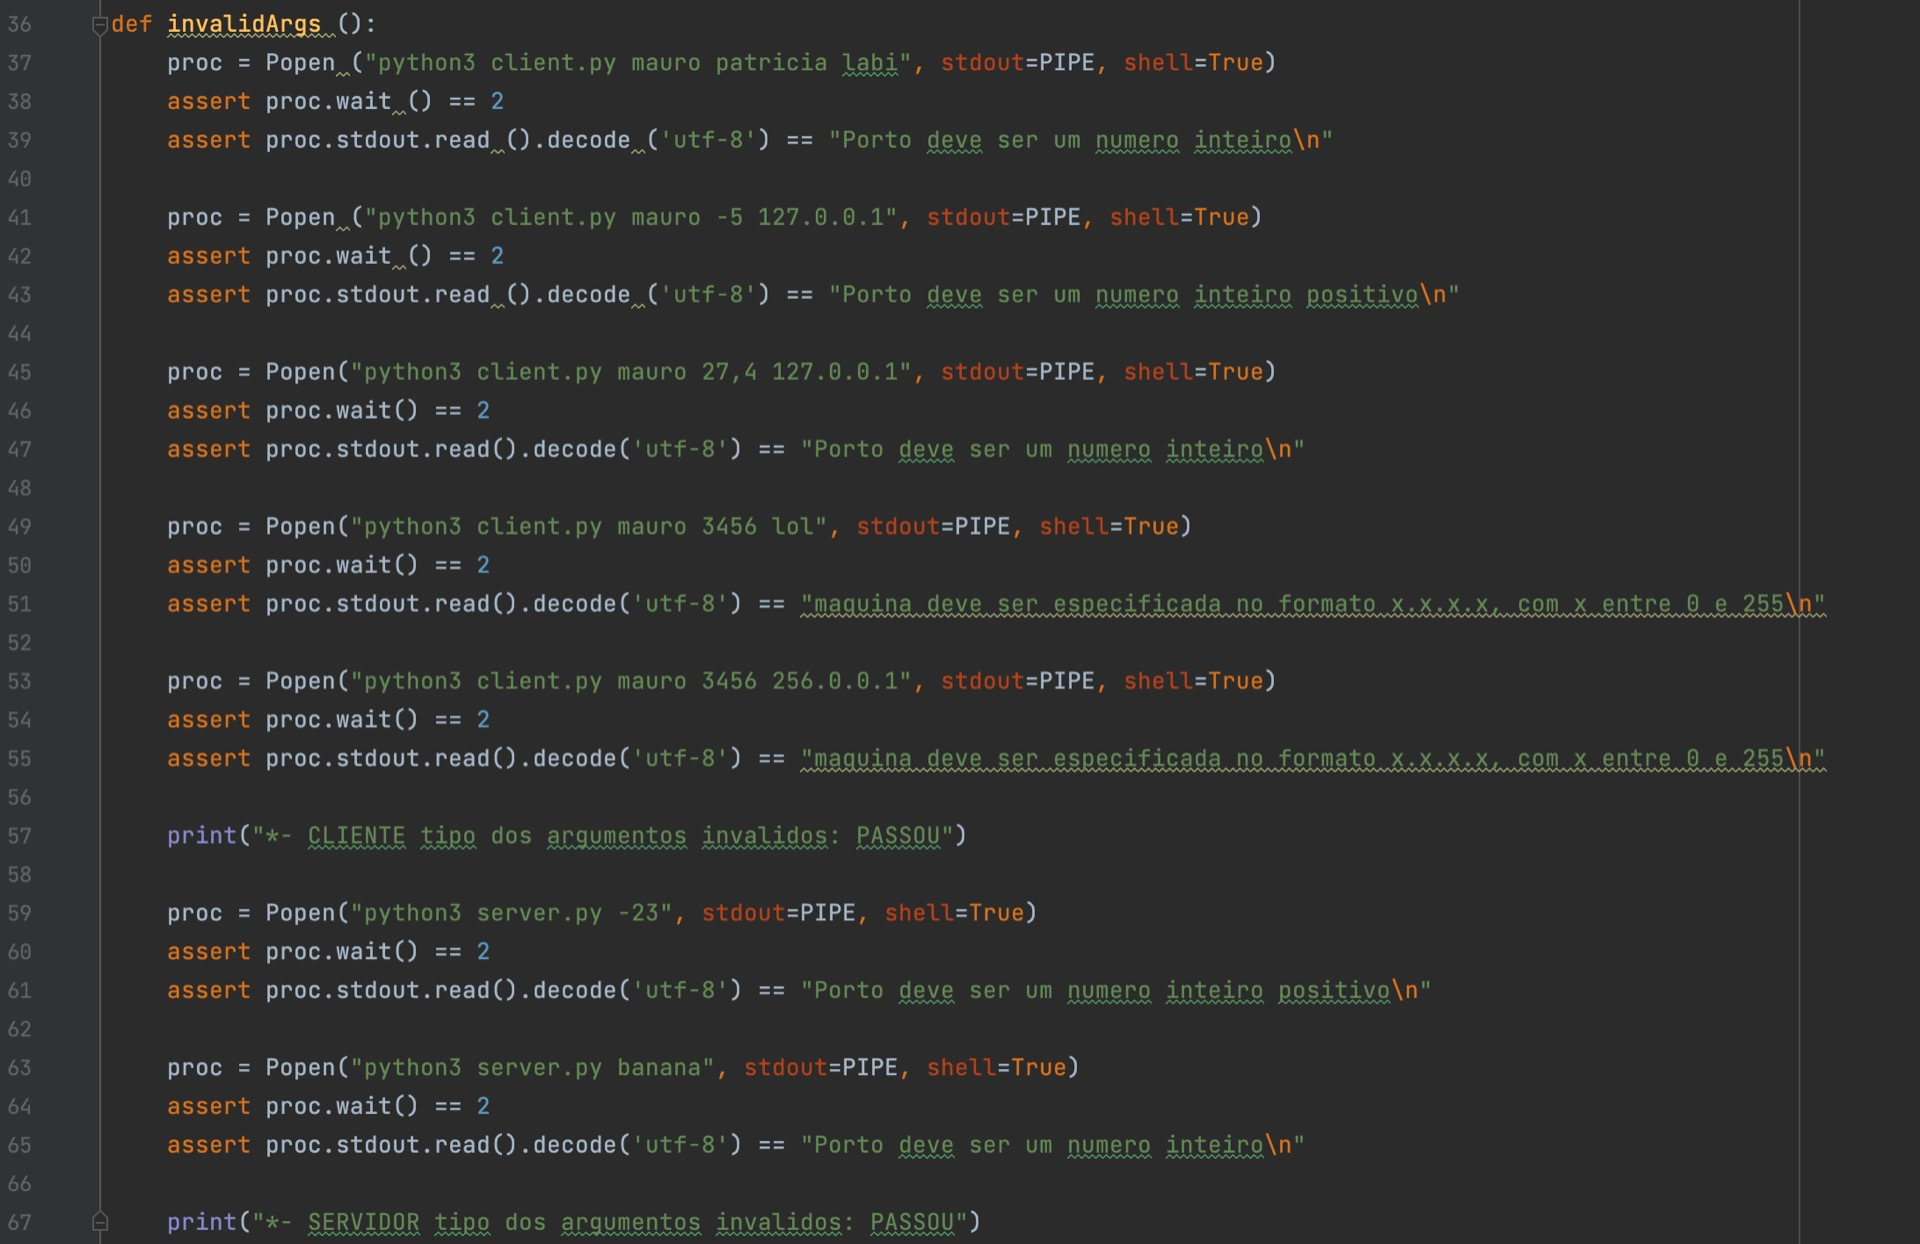
\includegraphics[scale=0.20]{testefuncional1}      
\end{figure}
Todos os erros relativos a tipos de argumentos inválidos implicam que a execução do programa termine, com código ‘2’. Por isso fazemos uma asserção para cada teste, de que o código retornado por ele deve ser também 2. A segunda asserção também implementada para testes dentro desta função, diz respeito à mensagem que é retornada pelo programa, quando identificada a falha. Caso a mensagem retornada, seja aquela que se esperava, então o programa lidou corretamente com as falhas.

\subsection{Teste unitário}
Para além dos testes funcionais, foi também desenvolvido, num ficheiro chamado ‘unitTests.py’, um simples teste unitário que vai testar as funções responsáveis por criptografar, e descriptografar, valores inteiros recebidos e enviados pelo programa cliente.
Para que o teste seja eficaz, utilizamos novamente o pacote ‘pytest’. Desta vez, para realizar o teste com precisão, também utilizamos os pacotes ‘os’ e ‘base64’, que irão gerar uma chave de cifra exatamente como aquela utilizada nos programas em que as funções aparecem.
\begin{figure}[H]
        \centering
        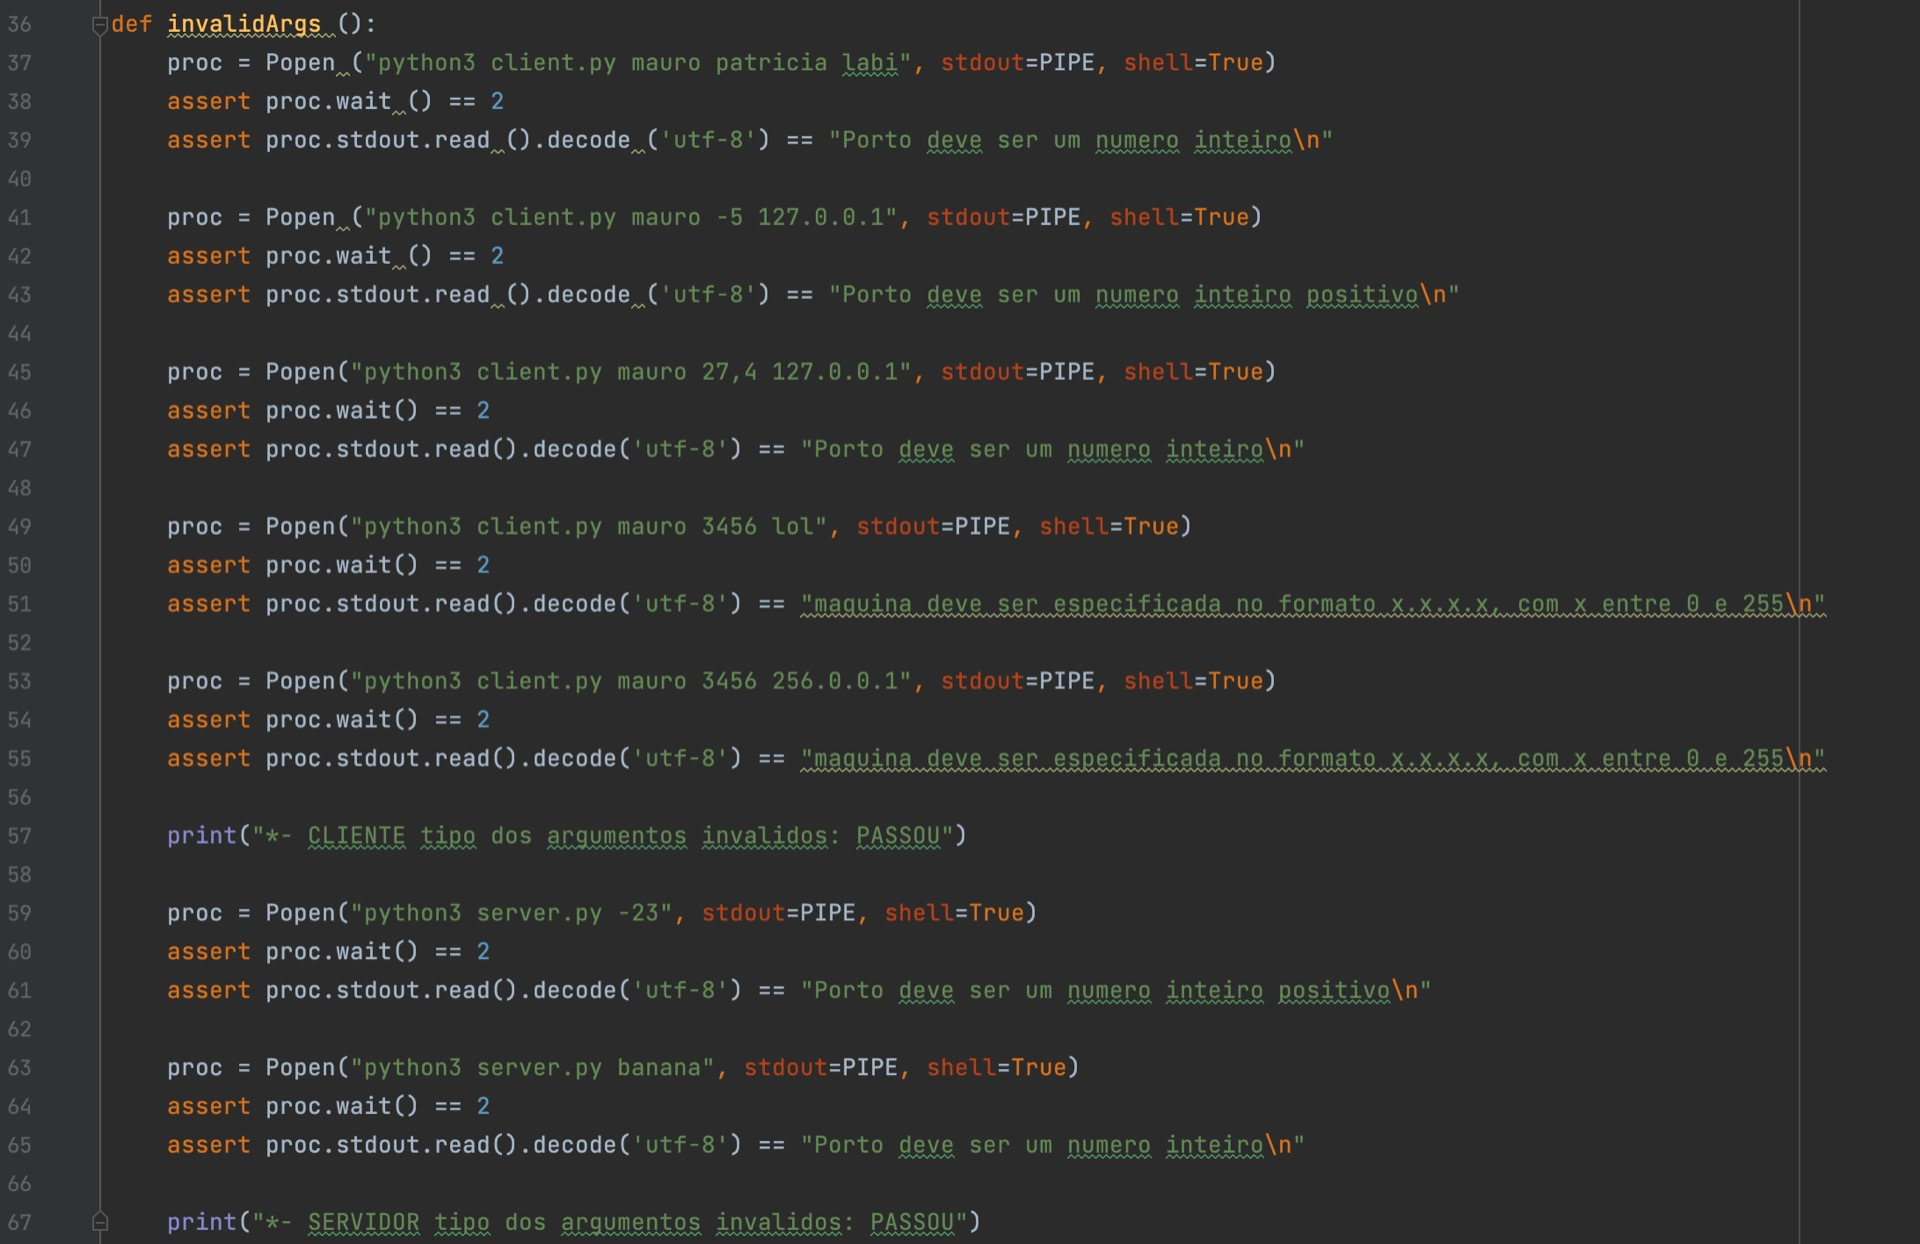
\includegraphics[scale=0.20]{testefuncional1}      
\end{figure}
Para que as funções passem este teste, encriptamos um número 1212, e depois o descriptografamos, recorrendo às funções aqui analisadas, e verificamos que o número retornado por elas após o processo de criptogra a é o mesmo. O que prova que as funções estão a
funcionar corretamente, ou não.

\chapter{Resultados/Análise}
\label{chap.resultados/análise}
Neste capítulo será apresentada a interação via terminal entre um ou mais clientes e o servidor.
\begin{itemize}
\item Jogo com um cliente e o servidor 
\begin{figure}[H]
        \centering
        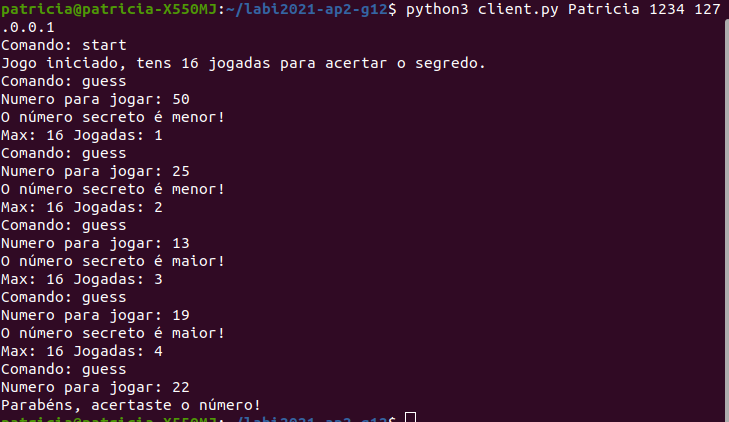
\includegraphics[scale=0.50]{guessNormal}      
        \caption{Terminal do cliente.}
\end{figure}

A aplicação está a funcionar de modo correto. É visível que quando o comando START é introduzido a aplicação indica que o jogo foi iniciado e exibe o número de tentativas que o cliente tem disponível para adivinhar o número secreto.
Depois, sempre que se introduz o comando GUESS, é pedido o palpite e ,após a introdução, é exibido se o número introduzido é maior, menor ou igual ao número secreto.E, também é mostrado o número de tentativas que ainda restam ao cliente para adivinhar o número secreto.

\begin{figure}[H]
        \centering
        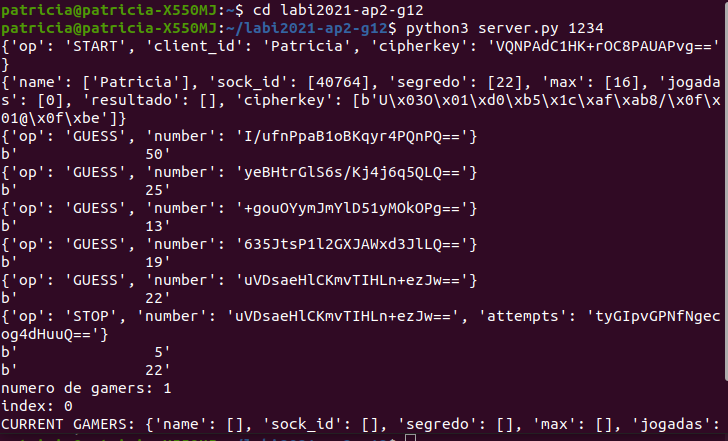
\includegraphics[scale=0.50]{guessNormal1}      
        \caption{Terminal do servidor.}
\end{figure}

O servidor está a acompanhar cada etapa executada pelo cliente. Por exemplo, quando o cliente introduziu o comando START é armazenado no dicionário os dados dos jogadores que estão ativos no jogo. Neste caso, o cliente Patrícia com o "sock\_id": 40764,o número secreto : 22, o número máximo de jogadas: 16, o número de jogadas efetuadas, o resultado e o tipo de cifragem.

\item Operação QUIT
\begin{figure}[H]
        \centering
        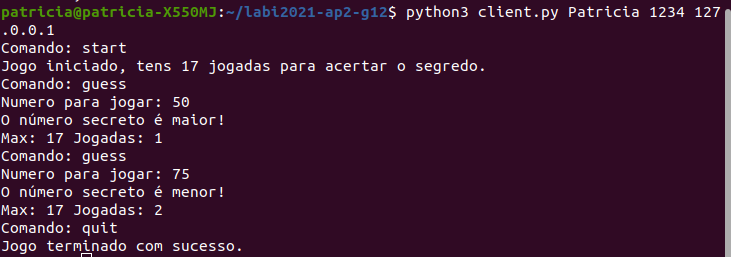
\includegraphics[scale=0.53]{guesscomquit}      
        \caption{Terminal do cliente.}
\end{figure}

A operação QUIT foi bem sucedida. Após a introdução do comando QUIT a mensagem exibida foi "Jogo terminado com sucesso" o que indica a desistência do cliente pois o número de tentativas ainda não tinha sido esgotado.

\begin{figure}[H]
        \centering
        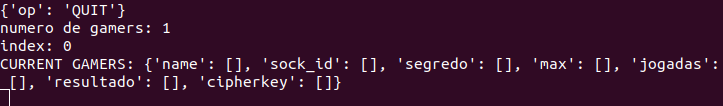
\includegraphics[scale=0.53]{guesscomquit1}      
        \caption{Terminal do servidor.}
\end{figure}

Após a operação QUIT ser executada o cliente é removido da lista de jogadores ativos.Assim, o dicionário encontra-se vazio pois não há nenhum cliente com um jogo iniciado.

\item Clientes com o mesmo client\_id
\begin{figure}[H]
        \centering
        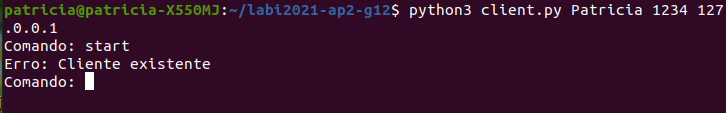
\includegraphics[scale=0.53]{mesmonome}      
        \caption{Ação da aplicação quando existem dois clientes com o mesmo id.}
\end{figure}

Havendo dois clientes com o mesmo client\_id a jogar ao mesmo tempo é de esperar que a aplicação exiba um erro a informar que já existe um cliente com esse id. Conclui-se que o programa está a funcionar corretamente pois é imprimida a mensagem "Erro: Cliente existente".

\item Clientes diferentes a jogar
\begin{figure}[H]
        \centering
        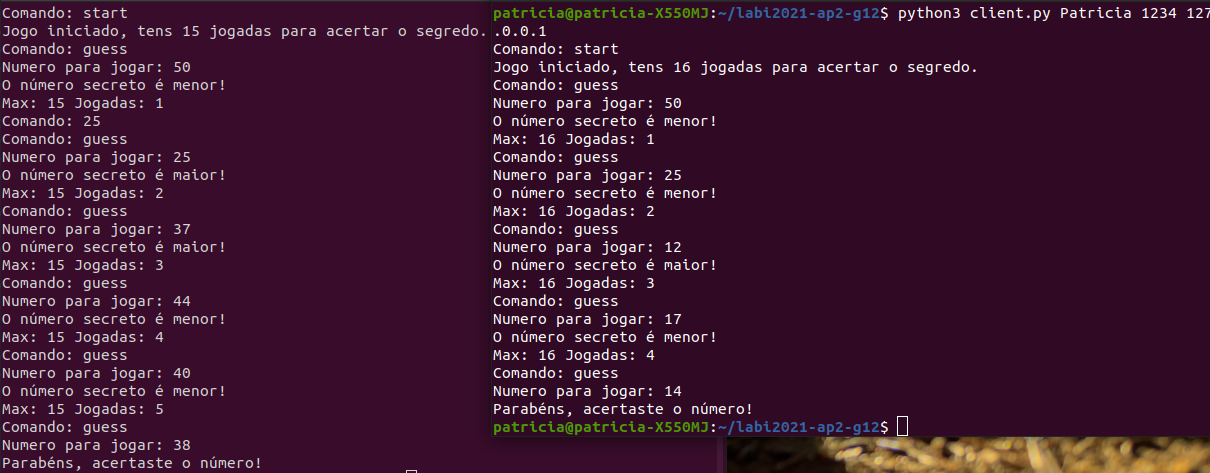
\includegraphics[scale=0.36]{doisclients}      
        \caption{Ação da aplicação quando existem dois clientes diferentes a jogar simultaneamente.}
\end{figure}

Neste caso, como o client\_id dos dois jogadores ativos é diferente a aplicação funciona corretamente, como seria de esperar, não havendo conflitos nem ocorrência de erros.

\item Introdução de comandos incorrectos
\begin{figure}[H]
        \centering
        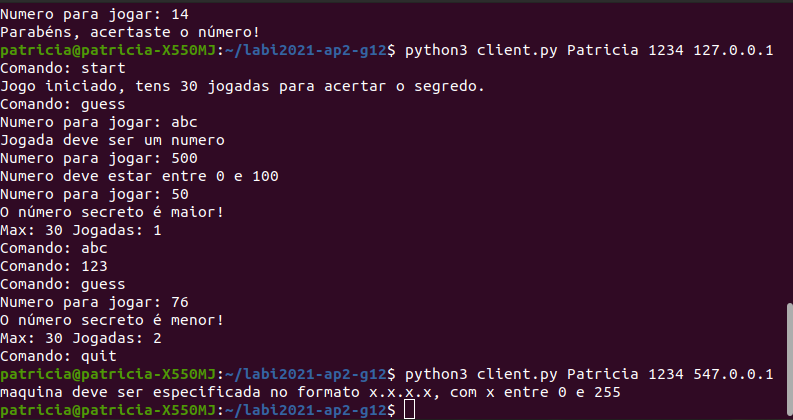
\includegraphics[scale=0.53]{errospropositados}      
        \caption{Comportamento da aplicação perante introdução de comandos incorrectos.}
\end{figure}

Após a introdução de uma string em vez de um número é exibida a mensagem "Jogada deve ser um numero".E, após a introdução de um número superior ao intervalo é imprido que o número deve estar entre 0 e 100. Para além disso, quando se coloca o nome/endereço da máquina incorretamente aparece a mensagem de erro "Maquina deve ser especificada no formato x.x.x.x, com x entre 0 e 255".

\item Armazenamento dos dados no ficheiro report.csv 
\begin{figure}[H]
        \centering
        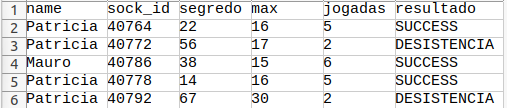
\includegraphics[scale=0.70]{ficheiro}      
        \caption{Ficheiro report.csv}
\end{figure}
O ficheiro report.csv foi atualizado corretamente com os dados dos jogadores ativos no jogo.

\end{itemize}


\chapter{Conclusões}
\label{chap.conclusao}

Durante o desenvolvimento deste projeto, pudemos colocar em prática vários conhecimentos que nos foram apresentados em aula durante o semestre, tais como: sockets, comunicação de mensagens TCP entre servidores e clientes, gravação de dados em ficheiros .CSV, criptografia, testes e depuração do código, entre outros mais.

O nosso objetivo com este projeto é desenvolver um jogo de adivinha o número, onde diversos clientes se podem conectar a um servidor que gerencia os jogos e armazena dados num cheiro .CSV. Este pode ser considerado um jogo simples em conceito, mas que requer esforço e dedicação para ser implementado de forma correta, clara e robusta.Os programas "client.py" e "server.py", acompanhados do pacote "common\_comm.py", formam juntos um jogo completo e totalmente funcional.

O cliente é capaz de gerenciar inputs do utilizador e executar pedidos ao servidor corretamente, recorrendo às suas várias funções anteriormente descritas, tendo a certeza de que todos os dados numéricos inteiros estão seguros por uma criptografia de ponta a ponta, que foi testada graças à implementação de um teste
unitário. O servidor por sua vez, recebe os pedidos dos vários possíveis clientes a jogar em simultâneo e é capaz de processá-los e devolver uma resposta ao cliente, criando assim uma interação completa e orgânica entre ambos os programas. Caso algo inesperado ocorra durante o jogo, os programas aqui desenvolvidos são programados para corrigir estas falhas sem consequências negativas. Por fim, a execução do jogo está também testada através de testes
funcionais, o que torna o projeto aqui escrito numa completa demonstração de conhecimento e aplicações práticas dos conteúdos desta cadeira.

Acreditamos não somente que atingimos a meta proposta para o trabalho, mas que também a excedemos em termos de aprendizagem prática. Todos os algoritmos, estratégias e motivos anteriormente descritos neste relatório constatam o longo caminho que percorremos
para alcançar o resultado final que é aqui apresentado com orgulho.
\chapter*{Contribuições dos autores}
Cada aluno fez o equivalente a cinquenta por cento.
\end{document}
